\documentclass{article}

% Required packages
\usepackage{amssymb}
\usepackage{amsmath}
\usepackage{graphicx}
\usepackage{geometry}
\usepackage{tikz}
\usepackage{array}
\usepackage{booktabs}
\usepackage{enumitem}
\usepackage{listings}
\usepackage{xcolor}
\usepackage{fancyhdr}
\usepackage{float}
\usepackage{subcaption}
\usepackage{comment}
\usepackage{algorithm}
\usepackage{algpseudocode}
\usepackage{booktabs}
\usepackage{caption}
\usepackage{subcaption}
\usepackage{booktabs}
\usepackage{array}
\usepackage{caption}
\usepackage{graphicx}
\usepackage{siunitx}
\usepackage{graphicx}
\usepackage{siunitx}
\usepackage{array}


% Set page geometry
\geometry{a4paper, margin=1in}

% Configure listings for Python
\lstset{
  language=Python,
  basicstyle=\ttfamily\footnotesize,
  numbers=left,
  numberstyle=\tiny\color{gray},
  frame=single,
  breaklines=true,
  breakatwhitespace=true,
  captionpos=b,
  tabsize=4,
  showspaces=false,
  showstringspaces=false,
  showtabs=false,
  commentstyle=\color{gray}\textit,
  keywordstyle=\color{blue}\bfseries,
  stringstyle=\color{red}
}

\begin{document}

\pagestyle{fancy}
\chead{DSC 257: Unsupervised Learning (Fall 2025)}
\lhead{Homework 4}
\rhead{Randall Rogers}

%------------------
% Solution for 1(a)
%------------------
\subsection*{Solution 1}
\noindent\rule{\textwidth}{0.4pt}\\
\subsubsection*{Solution 1 (a)}

Let $x = \begin{bmatrix}3 \\ 4\end{bmatrix}$.
To find the unit vector $u$, we must divide $x$ by its $L_2$-norm, $\|x\|_2 = \sqrt{x_1^2 + x_2^2}$.
\begin{align*}
    \|x\|_2 &= \sqrt{3^2 + 4^2} \\
            &= \sqrt{9 + 16} \\
            &= \sqrt{25} \\
            &= 5
\end{align*}
Now, we compute $u = \frac{x}{\|x\|_2}$.

\subsubsection*{\normalfont}{$\therefore$ the unit vector $u$ is the following:}
\begin{align*}
    u = \frac{1}{5} \begin{bmatrix}3 \\ 4\end{bmatrix} = \begin{bmatrix} 3/5 \\ 4/5 \end{bmatrix}
\end{align*}

\noindent\rule{\textwidth}{0.4pt}\\

\newpage

%------------------
% Solution for 1(b)
%------------------
\subsection*{Solution 1}
\noindent\rule{\textwidth}{0.4pt}\\
\subsubsection*{Solution 1 (b)}

Let $x = \begin{bmatrix}-4 \\ 12 \\ 3\end{bmatrix}$.
First, we find the $L_2$-norm of $x$, $\|x\|_2 = \sqrt{x_1^2 + x_2^2 + x_3^2}$.
\begin{align*}
    \|x\|_2 &= \sqrt{(-4)^2 + 12^2 + 3^2} \\
            &= \sqrt{16 + 144 + 9} \\
            &= \sqrt{169} \\
            &= 13
\end{align*}
The unit vector $u$ is $u = \frac{x}{\|x\|_2}$.

\subsubsection*{\normalfont}{$\therefore$ the unit vector $u$ is the following:}
\begin{align*}
    u = \frac{1}{13} \begin{bmatrix}-4 \\ 12 \\ 3\end{bmatrix} = \begin{bmatrix} \frac{-4}{13}  \\\\ \frac{12}{13} \\\\ \frac{3}{13} \end{bmatrix}
\end{align*}

\noindent\rule{\textwidth}{0.4pt}\\

\newpage

%------------------
% Solution for 1(c)
%------------------
\subsection*{Solution 1}
\noindent\rule{\textwidth}{0.4pt}\\
\subsubsection*{Solution 1 (c)}
Let $x = \begin{bmatrix}1 \\ 1 \\ \vdots \\ 1\end{bmatrix}$ such that $|x| = d$.
This vector consists of $d$ entries, each equal to 1. We find its $L_2$-norm:
\begin{align*}
    \|x\|_2 &= \sqrt{\sum_{i=1}^{d} 1^2} \\
            &= \sqrt{1 + 1 + \dots + 1} \quad (d \text{ times}) \\
            &= \sqrt{d}
\end{align*}
The unit vector $u$ is $u = \frac{x}{\|x\|_2}$.

\subsubsection*{\normalfont}{$\therefore$ the unit vector $u$ is the following:}
\begin{align*}
    u = \frac{1}{\sqrt{d}} \begin{bmatrix}1 \\ 1 \\ \vdots \\ 1\end{bmatrix} = \begin{bmatrix} \frac{1}{\sqrt{d}} \\ \frac{1}{\sqrt{d}} \\ \vdots \\ \frac{1}{\sqrt{d}} \end{bmatrix}
\end{align*}

\noindent\rule{\textwidth}{0.4pt}\\

\newpage

%------------------
% Solution for 2(a)
%------------------
\subsubsection*{Solution 2}
\noindent\rule{\textwidth}{0.4pt}\\
\subsubsection*{Solution 2 (a)}

Given point $x = \begin{bmatrix}-2 \\ 4\end{bmatrix}$ and direction $u = \begin{bmatrix}1 \\ 2\end{bmatrix}$.
The projection of vector $x$ onto vector $u$ is given by the formula:
$$\text{proj}_u x = \frac{x \cdot u}{\|u\|^2} u$$
\begin{flushleft}
  First, calculate the dot product $x \cdot u$:
\end{flushleft}

\begin{align*}
    x \cdot u &= (-2)(1) + (4)(2) \\
              &= -2 + 8 \\
              &= 6
\end{align*}
Next, calculate the squared $L_2$-norm of $u$, $\|u\|^2$:
\begin{align*}
    \|u\|^2 &= 1^2 + 2^2 \\
            &= 1 + 4 \\
            &= 5
\end{align*}
Now, substitute these values into the projection formula:
\begin{align*}
    \text{proj}_u x &= \frac{6}{5} \begin{bmatrix}1 \\ 2\end{bmatrix} \\
\end{align*}

\subsubsection*{\normalfont}{$\therefore$ the projection of point $x \in \mathbb{R}^2$ onto the direction of $u$ is: }
\begin{align*}
    \text{proj}_u x &= \begin{bmatrix} \frac{6}{5} \\\\ \frac{12}{5} \end{bmatrix} = \begin{bmatrix} 1.2 \\ 2.4 \end{bmatrix}
\end{align*}

\noindent\rule{\textwidth}{0.4pt}\\

\newpage

%------------------
% Solution for 2(b)
%------------------
\subsubsection*{Solution 2}
\noindent\rule{\textwidth}{0.4pt}\\
\subsubsection*{Solution 2 (b)}
\subsubsection*{Plot}
The projection is calculated to be:
$$\text{proj}_u x = \begin{bmatrix} 1.2 \\ 2.4 \end{bmatrix}$$

\begin{figure}[h!]
\centering
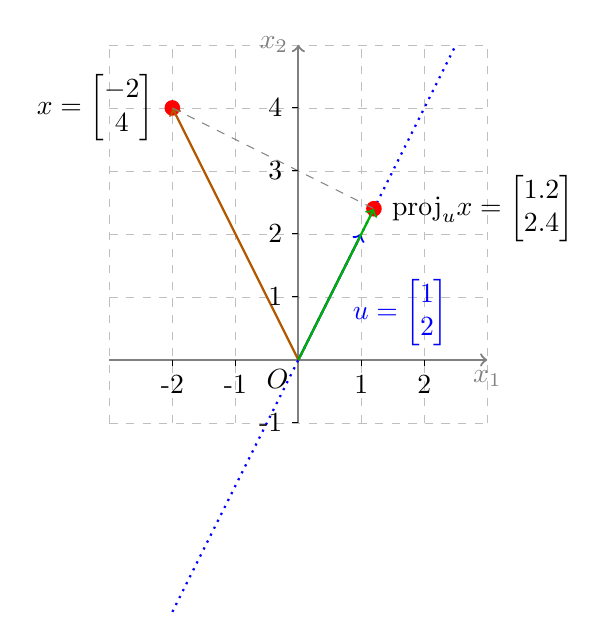
\begin{tikzpicture}[scale=0.8,
    axis_style/.style={->, thick, gray},
    vector_style/.style={->, thick, blue},
    point_style/.style={red, fill, circle, inner sep=2pt},
    projection_style/.style={->, thick, green!70!black},
    dashed_line/.style={dashed, gray}
]
    % Set up the grid
    \draw[help lines, dashed, opacity=0.5] (-3,-1) grid (3,5);

    % Draw axes
    \draw[axis_style] (-3,0) -- (3,0) node[below] {$x_1$};
    \draw[axis_style] (0,-1) -- (0,5) node[left] {$x_2$};

    % Mark origin
    \node at (0,0) [below left] {$O$};

    % Plot point x
    \node (x_point) at (-2,4) [point_style, label={left:$x=\begin{bmatrix}-2 \\ 4\end{bmatrix}$}] {};
    \draw[vector_style, orange!70!black] (0,0) -- (-2,4) node[above left, color=black, xshift=-0.2cm, yshift=0.2cm] {};

    % Plot direction u
    \draw[vector_style, blue] (0,0) -- (1,2) node[shift={(0.5, -1)}] {$u=\begin{bmatrix}1 \\ 2\end{bmatrix}$};
    % Extend the line for direction u for projection
    \draw[blue, thick, dotted] (-2,-4) -- (2.5,5); % Line representing the span of u

    % Plot the projection point
    \node (proj_point) at (1.2,2.4) [point_style, label={right:$\text{proj}_u x=\begin{bmatrix}1.2 \\ 2.4\end{bmatrix}$}] {};
    \draw[projection_style] (0,0) -- (1.2,2.4) node[below right, color=black, xshift=0.2cm, yshift=-0.2cm] {};

    % Draw the orthogonal line from x to its projection
    \draw[dashed_line] (-2,4) -- (1.2,2.4);

    % Add labels for coordinates
    \foreach \x in {-2,-1,1,2} \draw (\x,0) -- (\x,-0.1) node[below] {\x};
    \foreach \y in {-1,1,2,3,4} \draw (0,\y) -- (-0.1,\y) node[left] {\y};

\end{tikzpicture}
\caption{Projection of point $x$ onto direction $u$.}
\label{fig:projection_x_on_u}
\end{figure}

\noindent\rule{\textwidth}{0.4pt}\\

\newpage

%------------------
% Solution for 3(a)
%------------------
\subsubsection*{Solution 3}
\noindent\rule{\textwidth}{0.4pt}\\
\subsubsection*{Solution 3 (a)}
\subsubsection*{Maximized Projection}
Let, \\ 
$$x = \begin{bmatrix}-4 \\ 3\end{bmatrix}$$ \\
We can define the dot product as:
$$x \cdot u = |x||u|cos(\theta) \rightarrow \frac{x \cdot u}{|u|} = |x|cos(\theta)$$
The projection of $x$ onto a unit vector $u$ is:
$$\text{proj}_u x = \frac{x \cdot u}{\|u\|^2} u $$
Hence, the project of $x$ onto $u$ is maximized when $u$ is in the direction of $x$ or (i.e., $\theta=0$). \\
It follows that:
\begin{align*}
    \frac{x_1u1 + x_2u2}{\sqrt{u_{1}^{2}+u_{2}^{2}}} &= \sqrt{x_{1}^{2}+x_{2}^{2}}cos(\theta) \\
    \frac{-4u1 + 3u2}{\sqrt{u_{1}^{2}+u_{2}^{2}}} &= \sqrt{(-4)^{2}+3^{2}}\cos(0) \\
    \frac{-4u_1 + 3u_2}{\sqrt{u_{1}^{2}+u_{2}^{2}}} &= 5 \\
    \frac{-\frac{4u_1}{5} + \frac{3}{5}u_2}{\sqrt{u_{1}^{2}+u_{2}^{2}}} &= 1 \\
\end{align*}

\subsubsection*{\normalfont}{$\therefore$ the unit vector $u$ is the following:}

$$u = \begin{bmatrix} -\frac{4}{5} \\[4pt] \frac{3}{5} \end{bmatrix}$$

\noindent\rule{\textwidth}{0.4pt}\\

\newpage

%------------------
% Solution for 3(b)
%------------------
\subsubsection*{Solution 3}
\noindent\rule{\textwidth}{0.4pt}\\
\subsubsection*{Solution 3 (b)}
\subsubsection*{Minimized Projection}
Let, \\
$$x = \begin{bmatrix}-4 \\ 3\end{bmatrix}$$ \\
We can define the dot product as:
$$x \cdot u = \|x\|\,\|u\|\cos(\theta) \rightarrow \frac{x \cdot u}{\|u\|} = \|x\|\cos(\theta)$$
The projection of $x$ onto a unit vector $u$ is:
$$\text{proj}_u x = \frac{x \cdot u}{\|u\|^2} u.$$
Hence, the projection of $x$ onto $u$ is minimized when $u$ is opposite to $x$ (i.e., $\theta=\pi$). \\
It follows that:
\begin{align*}
    \frac{x_1u_1 + x_2u_2}{\sqrt{u_{1}^{2}+u_{2}^{2}}} &= \sqrt{x_{1}^{2}+x_{2}^{2}}\cos(\theta) \\
    \frac{-4u_1 + 3u_2}{\sqrt{u_{1}^{2}+u_{2}^{2}}} &= \sqrt{(-4)^{2}+3^{2}}\cos(\pi) \\
    \frac{-4u_1 + 3u_2}{\sqrt{u_{1}^{2}+u_{2}^{2}}} &= 5(-1) = -5 \\
    \frac{-\frac{4}{5}u_1 + \frac{3}{5}u_2}{\sqrt{u_{1}^{2}+u_{2}^{2}}} &= -1
\end{align*}

\subsubsection*{\normalfont}{$\therefore$ the unit vector $u$ is the following:}

$$u = \begin{bmatrix} \frac{4}{5} \\[2pt] -\frac{3}{5} \end{bmatrix}$$

\noindent\rule{\textwidth}{0.4pt}\\

\newpage

%------------------
% Solution for 3(c)
%------------------
\subsubsection*{Solution 3}
\noindent\rule{\textwidth}{0.4pt}\\
\subsubsection*{Solution 3 (c)}
\subsubsection*{Zero Projection}
Let, \\
$$x = \begin{bmatrix}-4 \\ 3\end{bmatrix}$$ \\
We can define the dot product as:
$$x \cdot u = \|x\|\,\|u\|\cos(\theta).$$
The projection of $x$ onto $u$ is zero when $x \cdot u = 0$ (i.e., $\theta \in\left\{\frac{\pi}{2}, \frac{3\pi}{2}\right\}$). For $u=\begin{bmatrix}u_1 \\ u_2\end{bmatrix}$,
\begin{align*}
    x \cdot u &= -4u_1 + 3u_2 = 0 \;\;\Longrightarrow\;\; 3u_2 = 4u_1 \;\;\Longrightarrow\;\; u_2 = \frac{4}{3}u_1.
\end{align*}
A direction orthogonal to $x$ is $v=\begin{bmatrix}3 \\ 4\end{bmatrix}$ since $x \cdot v = -12 + 12 = 0$, and $\|v\|=\sqrt{3^2+4^2}=5$. Normalizing yields the unit directions:
\begin{align*}
    u^{(1)} = \frac{1}{5}\begin{bmatrix}3 \\ 4\end{bmatrix} = \begin{bmatrix}\frac{3}{5} \\[2pt] \frac{4}{5}\end{bmatrix},
    \qquad
    u^{(2)} = -u^{(1)} = \begin{bmatrix}-\frac{3}{5} \\[2pt] -\frac{4}{5}\end{bmatrix}.
\end{align*}

\subsubsection*{\normalfont}{$\therefore$ the unit vector(s) $u$ are the following:}

$$u^{(1)} = \begin{bmatrix}\frac{3}{5} \\[4pt] \frac{4}{5}\end{bmatrix}
\quad \text{and} \quad
u^{(2)} = \begin{bmatrix}-\frac{3}{5} \\[4pt] -\frac{4}{5}\end{bmatrix}$$

\noindent\rule{\textwidth}{0.4pt}\\

\newpage

%------------------
% Solution for 4 (a)
%------------------
\subsubsection*{Solution 4}
\noindent\rule{\textwidth}{0.4pt}\\
\subsubsection*{Solution 4 (a)}
Let $\Sigma$ and direction $x$,
\[
\Sigma = \begin{bmatrix}
1 & 2 & 0 \\
2 & 9 & 0 \\
0 & 0 & 4
\end{bmatrix}
\qquad\text{and}\qquad
x = \begin{bmatrix}0 \\ 1 \\ 0\end{bmatrix}
\]
The variance in direction $x$ is $x^\top \Sigma x$.
\begin{align*}
\mathrm{Var}(x)
&= x^\top \Sigma x \\
&= \begin{bmatrix}0 & 1 & 0\end{bmatrix}
\begin{bmatrix}
1 & 2 & 0 \\
2 & 9 & 0 \\
0 & 0 & 4
\end{bmatrix}
\begin{bmatrix}0 \\ 1 \\ 0\end{bmatrix} \\
&= \begin{bmatrix}0 & 1 & 0\end{bmatrix}
\begin{bmatrix}
(1\cdot0) + (2\cdot1) + (0\cdot0) \\
(2\cdot0) + (9\cdot1) + (0\cdot0) \\
(0\cdot0) + (0\cdot1) + (4\cdot0)
\end{bmatrix} \\
&= \begin{bmatrix}0 & 1 & 0\end{bmatrix}
\begin{bmatrix}2 \\ 9 \\ 0\end{bmatrix}\\
&= (2\cdot0) + (9\cdot1) + (0\cdot0) \\
&= 9
\end{align*}
\subsubsection*{\normalfont}{$\therefore$ the variance in the direction $\begin{bmatrix}0 \\ 1 \\ 0\end{bmatrix}$ is $9$.}\\

\noindent\rule{\textwidth}{0.4pt}\\

\newpage

%------------------
% Solution for 4 (b)
%------------------
\subsubsection*{Solution 4}
\noindent\rule{\textwidth}{0.4pt}\\
\subsubsection*{Solution 4 (b)}
Let $\Sigma$ and unit direction $x$,
\[
\Sigma = \begin{bmatrix}
1 & 2 & 0 \\
2 & 9 & 0 \\
0 & 0 & 4
\end{bmatrix}
\qquad\text{and}\qquad
x = \frac{1}{\sqrt{3}}\begin{bmatrix}1 \\ 1 \\ 1\end{bmatrix}
\]
\begin{align*}
\mathrm{Var}(x)
&= x^\top \Sigma x \\
&= \left(\frac{1}{\sqrt{3}}\begin{bmatrix}1 & 1 & 1\end{bmatrix}\right)
\begin{bmatrix}
1 & 2 & 0 \\
2 & 9 & 0 \\
0 & 0 & 4
\end{bmatrix}
\left(\frac{1}{\sqrt{3}}\begin{bmatrix}1 \\ 1 \\ 1\end{bmatrix}\right) \\
&= \left(\frac{1}{\sqrt{3}} \cdot \frac{1}{\sqrt{3}}\right)
\begin{bmatrix}
(1\cdot1) + (2\cdot1) + (0\cdot1) \\
(2\cdot1) + (9\cdot1) + (0\cdot1) \\
(0\cdot1) + (0\cdot1) + (4\cdot1)
\end{bmatrix} \\
&= \frac{1}{3}\begin{bmatrix}1 & 1 & 1\end{bmatrix}
\begin{bmatrix}3 \\ 11 \\ 4\end{bmatrix}\\
&= \frac{1}{3}(3 + 11 + 4) \\
&= \frac{18}{3} \\
&= 6
\end{align*}

\subsubsection*{\normalfont}{$\therefore$ the variance in the direction $\frac{1}{\sqrt{3}}\begin{bmatrix}1 \\ 1 \\ 1\end{bmatrix}$ is $6$.} \\

\noindent\rule{\textwidth}{0.4pt}\\

\newpage

%------------------
% Solution for 4 (c)
%------------------
\subsubsection*{Solution 4}
\noindent\rule{\textwidth}{0.4pt}\\
\subsubsection*{Solution 4 (c)}
Let $\Sigma$ be as above and $u=\begin{bmatrix}u_1 \\ u_2 \\ u_3\end{bmatrix}\in\mathbb{R}^3$.
\begin{align*}
u^\top \Sigma u
&= \begin{bmatrix}u_1 & u_2 & u_3\end{bmatrix}
\begin{bmatrix}
1 & 2 & 0 \\
2 & 9 & 0 \\
0 & 0 & 4
\end{bmatrix}
\begin{bmatrix}u_1 \\ u_2 \\ u_3\end{bmatrix} \\
&= \begin{bmatrix}u_1 & u_2 & u_3\end{bmatrix}
\begin{bmatrix}u_1 + 2u_2 \\ 2u_1 + 9u_2 \\ 4u_3\end{bmatrix} \\
&= u_1(u_1 + 2u_2) + u_2(2u_1 + 9u_2) + u_3(4u_3) \\
&= u_1^2 + 4u_1u_2 + 9u_2^2 + 4u_3^2.
\end{align*}
Hence, we the form $a u_1^2 + b u_2^2 + c u_3^2 + d u_1 u_2$, and $a$,$b$,$c$,$d$ are:
\[
a = 1,\quad b = 9,\quad c = 4,\quad d = 4
\]
\subsubsection*{\normalfont}{$\therefore$ the variance function is:} 
$$u^\top\Sigma u = u_1^2 + 4u_1u_2 + 9u_2^2 + 4u_3^2$$

\noindent\rule{\textwidth}{0.4pt}\\

\newpage

%------------------
% Solution for 5
%------------------
\subsubsection*{Solution 5}
\noindent\rule{\textwidth}{0.4pt}\\
\subsubsection*{Solution 5}
Let $\Sigma$,
\[
\Sigma =
\begin{bmatrix}
    5 & 0 & 0 & 0 & 0 \\
    0 & 10 & 0 & 0 & 0 \\
    0 & 0 & 20 & 0 & 0 \\
    0 & 0 & 0 & 1 & 0 \\
    0 & 0 & 0 & 0 & 4 \\
\end{bmatrix}
\]
For any unit direction $u=\begin{bmatrix}u_1\\u_2\\u_3\\u_4\\u_5\end{bmatrix}\in\mathbb{R}^5$ with $\|u\|_2=1$, the variance in direction $u$ is
\begin{align*}
\mathrm{Var}(u) &= u^\top \Sigma u \\
&=
\begin{bmatrix}
  u_1 & u_2 & u_3 & u_4 & u_5 
\end{bmatrix}
\begin{bmatrix}
    5 & 0 & 0 & 0 & 0 \\
    0 & 10 & 0 & 0 & 0 \\
    0 & 0 & 20 & 0 & 0 \\
    0 & 0 & 0 & 1 & 0 \\
    0 & 0 & 0 & 0 & 4 
\end{bmatrix}
\begin{bmatrix}u_1\\u_2\\u_3\\u_4\\u_5\end{bmatrix}\\
% First, multiply the matrix \Sigma by the vector u
&=
\begin{bmatrix}
  u_1 & u_2 & u_3 & u_4 & u_5 
\end{bmatrix}
\begin{bmatrix}
    (5u_1 + 0u_2 + 0u_3 + 0u_4 + 0u_5) \\
    (0u_1 + 10u_2 + 0u_3 + 0u_4 + 0u_5) \\
    (0u_1 + 0u_2 + 20u_3 + 0u_4 + 0u_5) \\
    (0u_1 + 0u_2 + 0u_3 + 1u_4 + 0u_5) \\
    (0u_1 + 0u_2 + 0u_3 + 0u_4 + 4u_5)
\end{bmatrix} \\
&=
\begin{bmatrix}
  u_1 & u_2 & u_3 & u_4 & u_5 
\end{bmatrix}
\begin{bmatrix}
    5u_1 \\
    10u_2 \\
    20u_3 \\
    1u_4 \\
    4u_5
\end{bmatrix}\\
% Now, perform the final dot product
&= u_1(5u_1) + u_2(10u_2) + u_3(20u_3) + u_4(1u_4) + u_5(4u_5) \\
&= 5u_1^2 + 10u_2^2 + 20u_3^2 + u_4^2 + 4u_5^2
\end{align*}

\subsubsection*{\normalfont}{$\therefore$ the direction of maximum variance is: 
$$u=\begin{bmatrix}0\\0\\1\\0\\0\end{bmatrix}$$ 

\noindent\rule{\textwidth}{0.4pt}\\

\newpage

%------------------
% Solution for 6 (a)
%------------------
\subsubsection*{Solution 6}
\noindent\rule{\textwidth}{0.4pt}\\
\subsubsection*{Solution 6 (a)}
\subsubsection*{Mean and Variance of $X\cdot u$}
Let,
 $$\mu = \mathbb{E}[X] = \begin{bmatrix}1 \\ 2 \\ 3\end{bmatrix} \text{  and   } \Sigma=\operatorname{cov}(X)=
\begin{bmatrix}
5 & -3 & 0 \\
-3 & 5 & 0 \\
0 & 0 & 4
\end{bmatrix} \text{  and   } u=\dfrac{1}{\sqrt{3}}\begin{bmatrix}1 \\ 1 \\ 1\end{bmatrix}$$
\begin{align*}
\mathbb{E}[X\cdot u] &= u^\top \mu \\
&= \frac{1}{\sqrt{3}}\begin{bmatrix}1 & 1 & 1\end{bmatrix}\begin{bmatrix}1 \\ 2 \\ 3\end{bmatrix} \\
&= \frac{1}{\sqrt{3}}(1+2+3) \\
&= \frac{6}{\sqrt{3}}\\\\
\operatorname{Var}(X\cdot u) &= u^\top \Sigma u \\
&= \left(\frac{1}{\sqrt{3}}\begin{bmatrix}1 & 1 & 1\end{bmatrix}\right)
\begin{bmatrix}
5 & -3 & 0 \\
-3 & 5 & 0 \\
0 & 0 & 4
\end{bmatrix}
\left(\frac{1}{\sqrt{3}}\begin{bmatrix}1 \\ 1 \\ 1\end{bmatrix}\right) \\
&= \frac{1}{3}\begin{bmatrix}1 & 1 & 1\end{bmatrix}\begin{bmatrix}2 \\ 2 \\ 4\end{bmatrix} \\
&= \frac{1}{3}(2+2+4) \\
&= \frac{8}{3}
\end{align*}
\subsubsection*{\normalfont}{$\therefore$ $\mathbb{E}[X\cdot u]=\frac{6}{\sqrt{3}}$ and $\operatorname{Var}(X\cdot u)=\dfrac{8}{3}$.}

\noindent\rule{\textwidth}{0.4pt}\\

\newpage

%------------------
% Solution for 6 (b)
%------------------
\subsubsection*{Solution 6}
\noindent\rule{\textwidth}{0.4pt}\\
\subsubsection*{Solution 6 (b)}
Let
\[
\Sigma=\begin{bmatrix}
5 & -3 & 0\\
-3 & 5 & 0\\
0 & 0 & 4
\end{bmatrix},
\quad
v_1=\begin{bmatrix}1\\0\\0\end{bmatrix},\;
v_2=\begin{bmatrix}0\\1\\0\end{bmatrix},\;
v_3=\begin{bmatrix}0\\0\\1\end{bmatrix},
\]
\[
v_4=\frac{1}{\sqrt{2}}\begin{bmatrix}1\\1\\0\end{bmatrix},\;
v_5=\frac{1}{\sqrt{2}}\begin{bmatrix}0\\1\\1\end{bmatrix},\;
v_6=\frac{1}{\sqrt{2}}\begin{bmatrix}1\\-1\\0\end{bmatrix}
\]
Check each candidate via $\Sigma v=\lambda v$:

\begin{align*}
\Sigma v_1 &= \begin{bmatrix}5\\-3\\0\end{bmatrix}&
&\neq \lambda \begin{bmatrix}1\\0\\0\end{bmatrix}\;\text{for any }\lambda
&\quad \Longrightarrow\quad v_1\ \text{is not an eigenvector}.\\[6pt]
\Sigma v_2 &= \begin{bmatrix}-3\\5\\0\end{bmatrix}&
&\neq \lambda \begin{bmatrix}0\\1\\0\end{bmatrix}\;\text{for any }\lambda
&\quad\Longrightarrow\quad v_2\ \text{is not an eigenvector}.\\[6pt]
\Sigma v_3 &= \begin{bmatrix}0\\0\\4\end{bmatrix}&
&= 4\begin{bmatrix}0\\0\\1\end{bmatrix}
&\quad\Longrightarrow\quad v_3\ \text{is an eigenvector with }\lambda=4.\\[6pt]
\Sigma v_4 &= \frac{1}{\sqrt{2}}\begin{bmatrix}2\\2\\0\end{bmatrix}&
&= 2\left(\frac{1}{\sqrt{2}}\begin{bmatrix}1\\1\\0\end{bmatrix}\right)
&\quad\Longrightarrow\quad v_4\ \text{is an eigenvector with }\lambda=2.\\[6pt]
\Sigma v_5 &= \frac{1}{\sqrt{2}}\begin{bmatrix}-3\\5\\4\end{bmatrix}&
&\neq \lambda \left(\frac{1}{\sqrt{2}}\begin{bmatrix}0\\1\\1\end{bmatrix}\right)\ \text{for any }\lambda
&\quad\Longrightarrow\quad v_5\ \text{is not an eigenvector}.\\[6pt]
\Sigma v_6 &= \frac{1}{\sqrt{2}}\begin{bmatrix}8\\-8\\0\end{bmatrix}&
&= 8\left(\frac{1}{\sqrt{2}}\begin{bmatrix}1\\-1\\0\end{bmatrix}\right)
&\quad\Longrightarrow\quad v_6\ \text{is an eigenvector with }\lambda=8.
\end{align*}

\subsubsection*{\normalfont}{$\therefore$ From the provided list, the eigenvectors are:}
$$\dfrac{1}{\sqrt{2}}\begin{bmatrix}1\\1\\0\end{bmatrix}\text{ with eigenvalue } 2\text{, } \dfrac{1}{\sqrt{2}}\begin{bmatrix}1\\-1\\0\end{bmatrix}\text{ with eigenvalue }8\text{, and }\begin{bmatrix}0\\0\\1\end{bmatrix} \text{ with eigenvalue } 4$$

\noindent\rule{\textwidth}{0.4pt}\\

\newpage

%------------------
% Solution for 6 (c)
%------------------
\subsubsection*{Solution 6}
\noindent\rule{\textwidth}{0.4pt}\\
\subsubsection*{Solution 6 (c)}
\subsubsection*{Eigenvalues for the eigenvectors from (b)}
From the computations in (b),

$$\lambda\!\left(\tfrac{1}{\sqrt{2}}\begin{bmatrix}1 \\ 1 \\ 0\end{bmatrix}\right)=2,\quad \text{eigenvalue: } 2$$\\
$$\lambda\!\left(\tfrac{1}{\sqrt{2}}\begin{bmatrix}1 \\ -1 \\ 0\end{bmatrix}\right)=8,\quad \text{eigenvalue: } 8$$ \\
$$\lambda\!\left(\begin{bmatrix}0 \\ 0 \\ 1\end{bmatrix}\right)=4, \quad \text{eigenvalue: } 4$$ \\

\noindent\rule{\textwidth}{0.4pt}\\

\newpage

%------------------
% Solution for 6 (d)
%------------------
\subsubsection*{Solution 6}
\noindent\rule{\textwidth}{0.4pt}\\
\subsubsection*{Solution 6 (d)}
\subsubsection*{PCA: 2D projection directions}
Eigenvalues (descending) are $8,4,2$. Thus the top two principal directions are the eigenvectors for $8$ and $4$:
\[
v_1=\frac{1}{\sqrt{2}}\begin{bmatrix}1 \\ -1 \\ 0\end{bmatrix},\qquad
v_2=\begin{bmatrix}0 \\ 0 \\ 1\end{bmatrix}.
\]
\subsubsection*{\normalfont}{$\therefore$ PCA projects onto $\left\{\tfrac{1}{\sqrt{2}}\begin{bmatrix}1 \\ -1 \\ 0\end{bmatrix},\;\begin{bmatrix}0 \\ 0 \\ 1\end{bmatrix}\right\}$}\\

\noindent\rule{\textwidth}{0.4pt}\\

\newpage

%------------------
% Solution for 6 (e)
%------------------
\subsubsection*{Solution 6}
\noindent\rule{\textwidth}{0.4pt}\\
\subsubsection*{Solution 6 (e)}
\subsubsection*{2D PCA projection}
Let, \\
$$x=\begin{bmatrix}4 \\ 0 \\ 2\end{bmatrix} \quad \mu = \begin{bmatrix}1 \\ 2 \\ 3\end{bmatrix} \quad v_1=\tfrac{1}{\sqrt{2}}\begin{bmatrix}1 \\ -1 \\ 0\end{bmatrix} \quad v_2=\begin{bmatrix}0 \\ 0 \\ 1\end{bmatrix}$$ \\

\begin{enumerate}
  \item Center $x$ by $\mu$
  $$x-\mu=\begin{bmatrix}4-1 \\ 0-2 \\ 2-3\end{bmatrix}=\begin{bmatrix}3 \\ -2 \\ -1\end{bmatrix}$$
  \item Find $y_1$
  \begin{align*}
    y_1 &= v_1^\top (x-\mu) \\
    &= \frac{1}{\sqrt{2}}\begin{bmatrix}1 & -1 & 0\end{bmatrix}\begin{bmatrix}3 \\ -2 \\ -1\end{bmatrix} \\
    &= \frac{1}{\sqrt{2}}(3+2) \\
    &= \frac{5}{\sqrt{2}} \\
  \end{align*}
  \item Find $y_2$
  \begin{align*}
    y_2 &= v_2^\top (x-\mu) \\
    &= \begin{bmatrix}0 & 0 & 1\end{bmatrix}\begin{bmatrix}3 \\ -2 \\ -1\end{bmatrix} \\
    &= -1
  \end{align*}
\end{enumerate}

\subsubsection*{\normalfont}{$\therefore$ The 2D PCA coordinates are $\begin{bmatrix}\dfrac{5}{\sqrt{2}} \\[10pt] -1\end{bmatrix}$}

\noindent\rule{\textwidth}{0.4pt}\\

\newpage

%------------------
% Solution for 6 (f)
%------------------
\subsubsection*{Solution 6}
\noindent\rule{\textwidth}{0.4pt}\\
\subsubsection*{Solution 6 (f)}
\subsubsection*{Reconstruction from 2D PCA}
Let, \\
$$\mu = \begin{bmatrix}1 \\ 2 \\ 3\end{bmatrix} \quad y_1 = \frac{5}{\sqrt{2}} \quad y_2 = -1 \quad v_1=\tfrac{1}{\sqrt{2}}\begin{bmatrix}1 \\ -1 \\ 0\end{bmatrix} \quad v_2=\begin{bmatrix}0 \\ 0 \\ 1\end{bmatrix}$$ \\

\begin{align*}
x &= \mu + y_1 v_1 + y_2 v_2\\
&= \begin{bmatrix}1 \\ 2 \\ 3\end{bmatrix}
+ \frac{5}{\sqrt{2}}\left(\frac{1}{\sqrt{2}}\begin{bmatrix}1 \\ -1 \\ 0\end{bmatrix}\right)
+ (-1)\begin{bmatrix}0 \\ 0 \\ 1\end{bmatrix} \\
&= \begin{bmatrix}1 \\ 2 \\ 3\end{bmatrix}
+ \frac{5}{2}\begin{bmatrix}1 \\ -1 \\ 0\end{bmatrix}
+ \begin{bmatrix}0 \\ 0 \\ -1\end{bmatrix}\\
&= \begin{bmatrix}1+\frac{5}{2} \\ 2-\frac{5}{2} \\ 3-1\end{bmatrix}\\
&= \begin{bmatrix}\frac{7}{2} \\-\frac{1}{2} \\ 2\end{bmatrix}
\end{align*}
\subsubsection*{\normalfont}{$\therefore$ The 3D reconstruction is:}

$$x=\begin{bmatrix}\tfrac{7}{2} \\[6pt] -\tfrac{1}{2} \\[6pt] 2\end{bmatrix}$$

\noindent\rule{\textwidth}{0.4pt}\\

\newpage

\subsubsection*{Solution 7}
\noindent\rule{\textwidth}{0.4pt}
\subsubsection*{Solution 7 (a)}
\subsubsection*{PCA 2D Projection}

\begin{figure}[h]
  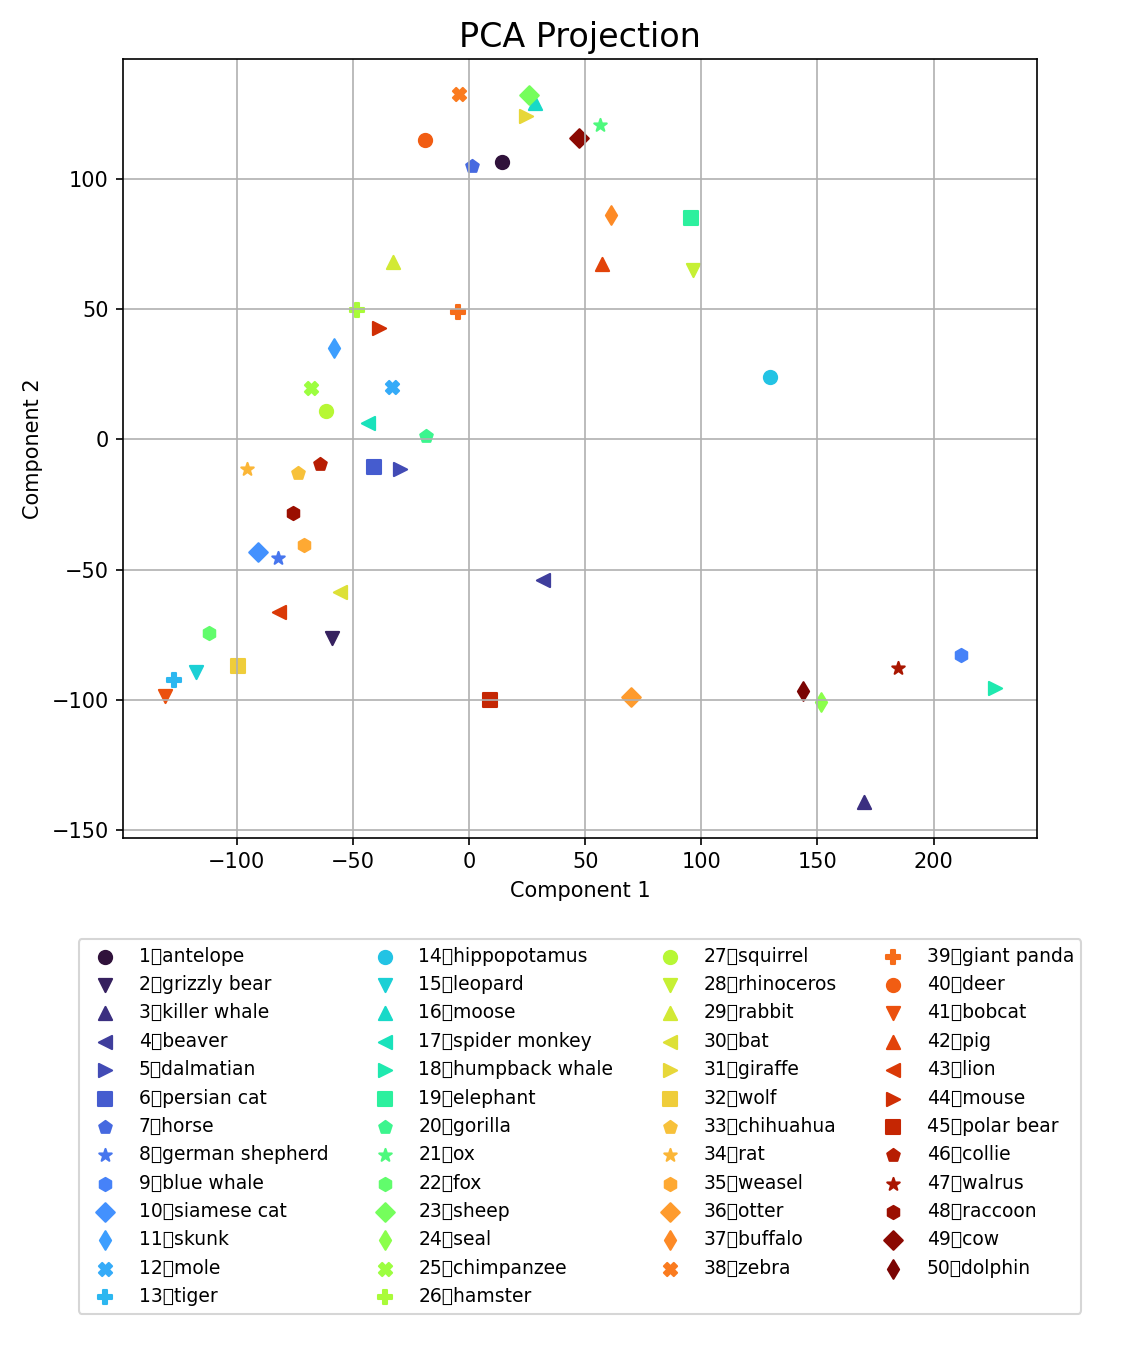
\includegraphics[height=0.75\textheight,width=\textwidth]{pca_projection.png}
  \caption{PCA projection $\mathbb{R}^{85}$ to $\mathbb{R}^{2}$}
\end{figure}
\noindent\rule{\textwidth}{0.4pt}\\

\newpage

\subsubsection*{Solution 7}
\noindent\rule{\textwidth}{0.4pt}
\subsubsection*{Solution 7 (a)}
\subsubsection*{PCA Code}
\begin{lstlisting}
import numpy as np
import matplotlib.pyplot as plt
from sklearn.decomposition import PCA
from sklearn.manifold import TSNE
from scipy.spatial.distance import pdist, squareform
import re 

# set plot figure size for better readability 
plt.rcParams['figure.figsize'] = (6, 8)

def load_animal_names(filepath='classes.txt'):
    with open(filepath, 'r') as f:
        names = [line.strip() for line in f.readlines()]
        names = [name.split('.')[-1].replace('+', ' ') for name in names]
    return(names)

def main():
    # read predicate-matrix-continuous.txt
    X = np.loadtxt('predicate-matrix-continuous.txt')
    # read classes.txt
    animal_names = load_animal_names('classes.txt')
    
    # initalize list to hold embeddings and their titles
    embeddings_to_plot = []
    # pca model
    pca = PCA(n_components=2, random_state=42)
    Z_pca = pca.fit_transform(X)
    embeddings_to_plot.append(('PCA Projection', Z_pca))
\end{lstlisting}

\newpage

\subsubsection*{Solution 7}
\noindent\rule{\textwidth}{0.4pt}
\subsubsection*{Solution 7 (b)}
\subsubsection*{t-SNE Code}
\begin{lstlisting}
import numpy as np
import matplotlib.pyplot as plt
from sklearn.decomposition import PCA
from sklearn.manifold import TSNE
from scipy.spatial.distance import pdist, squareform
import re 

# set plot figure size for better readability 
plt.rcParams['figure.figsize'] = (6, 8)

def load_animal_names(filepath='classes.txt'):
    with open(filepath, 'r') as f:
        names = [line.strip() for line in f.readlines()]
        names = [name.split('.')[-1].replace('+', ' ') for name in names]
    return(names)

def main():
    # read predicate-matrix-continuous.txt
    X = np.loadtxt('predicate-matrix-continuous.txt')
    # read classes.txt
    animal_names = load_animal_names('classes.txt')
    
    # initalize list to hold embeddings and their titles
    embeddings_to_plot = []
    
    # note: 49 ~ 50 its just python indexing
    perplexities = [5, 10, 25, 49]
    for p in perplexities:
        print(f"Running t-SNE with perplexity={p}...")
        tsne = TSNE(n_components=2, perplexity=p, random_state=42, 
                    init='pca', learning_rate='auto')
        Z_tsne = tsne.fit_transform(X)
        embeddings_to_plot.append((f't-SNE (Perplexity={p})', Z_tsne))
\end{lstlisting}

\newpage

\subsubsection*{Solution 7}
\noindent\rule{\textwidth}{0.4pt}
\subsubsection*{Solution 7 (c)}
\subsubsection*{Evaluate Models}

\noindent\rule{\textwidth}{0.4pt}
\begin{table}[h]
\centering

%\label{tab:distortion_analysis}

\begin{tabular}{llr}
\toprule
\textbf{Plot} & \textbf{Description} & \textbf{Average Distortion} \\
\midrule
\texttt{pca\_projection.png} & PCA Projection & 1.8313 \\
\texttt{t\_sne\_perplexity5.png} & t-SNE (Perplexity=5) & 1.8602 \\
\texttt{t\_sne\_perplexity10.png} & t-SNE (Perplexity=10) & 1.7101 \\
\texttt{t\_sne\_perplexity25.png} & t-SNE (Perplexity=25) & 1.5683 \\
\texttt{t\_sne\_perplexity49.png} & t-SNE (Perplexity=49) & 1.7370 \\
\bottomrule
\end{tabular}

\vspace{1em}
\caption[Distortion Analysis]{The embedding with the lowest average distortion is t-SNE (Perplexity=25) with a minimum distortion of 1.5683.}
\label{tab:distortion_analysis}

\end{table}

\newpage

\subsubsection*{Solution 7}
\noindent\rule{\textwidth}{0.4pt}
\subsubsection*{Solution 7 (c)}
\subsubsection*{Distortion and Plot Code}
\begin{lstlisting}
import numpy as np
import matplotlib.pyplot as plt
from sklearn.decomposition import PCA
from sklearn.manifold import TSNE
from scipy.spatial.distance import pdist, squareform
import re 

# set plot figure size for better readability 
plt.rcParams['figure.figsize'] = (6, 8)

def load_animal_names(filepath='classes.txt'):
    with open(filepath, 'r') as f:
        names = [line.strip() for line in f.readlines()]
        names = [name.split('.')[-1].replace('+', ' ') for name in names]
    return(names)

def compute_distortion(X_original, Z_embedded):
    # calc pairwise distances for original space (n*(n-1)/2 vector)
    D = pdist(X_original, metric='euclidean')

    # calc pairwise distances for embedded space (n*(n-1)/2 vector)
    D_hat = pdist(Z_embedded, metric='euclidean')
    
    # add a small epsilon to avoid division by zero
    epsilon = 1e-12
    D[D == 0] = epsilon
    D_hat[D_hat == 0] = epsilon
    
    # calc scaling factor c (sum of all pairwise distances)
    c = np.sum(D) / np.sum(D_hat)
    
    # calc scaled embedded distances
    scaled_D_hat = c * D_hat
    
    # calculate distortion for each pair (i, j) with i < j
    Delta_values = np.maximum(D / scaled_D_hat, scaled_D_hat / D)
    
    return(np.mean(Delta_values))

def main():
    # read predicate-matrix-continuous.txt
    X = np.loadtxt('predicate-matrix-continuous.txt')
    # read classes.txt
    animal_names = load_animal_names('classes.txt')
    
    # initalize list to hold embeddings and their titles
    embeddings_to_plot = []
    
    for title, Z in embeddings_to_plot:
        # set plt configs
        fig = plt.figure(figsize=(7.5, 9))
        grid_shape = (3, 3)
        ax_plot = plt.subplot2grid(grid_shape, (0, 0), rowspan=2, colspan=3)
        ax_legend = plt.subplot2grid(grid_shape, (2, 0), rowspan=1, colspan=3)
        
        # plot data
        for j, name in enumerate(animal_names):
            color = colors[j]
            marker = markers[j % len(markers)]
            
            ax_plot.scatter(Z[j, 0], Z[j, 1], 
                            color=color, 
                            marker=marker, 
                            label=name, 
                            s=40) # s=40 is a reasonable marker size
        
        ax_plot.set_title(title, fontsize=16)
        ax_plot.set_xlabel('Component 1')
        ax_plot.set_ylabel('Component 2')
        ax_plot.grid(True)
        
        # set legend settings
        handles, labels = ax_plot.get_legend_handles_labels()
        ax_legend.axis('off')
        ax_legend.legend(handles, labels, loc='center', ncol=4, fontsize=9)
        
        # save plot
        # Use tight_layout to ensure no overlap
        plt.tight_layout()
        clean_title = title.lower()
        clean_title = re.sub(r'[^\w\s-]', '', clean_title) 
        clean_title = re.sub(r'[\s-]+', '_', clean_title).strip('_')
        filename = f"{clean_title}.png"
        
        plt.savefig(filename, dpi=150) # 150 dpi is good for print
        plt.close(fig) # Close the figure to free memory

    # calc distortion
    distortions = {}
    
    # store all embeddings in a dict for distortion calculation
    all_embeddings_dict = {title: Z for title, Z in embeddings_to_plot}
        
    for key, Z in all_embeddings_dict.items():
        distortion = compute_distortion(X, Z)
        distortions[key] = distortion
        print(f"{key} average distortion: {distortion:.4f}")
        
    best_embedding = min(distortions, key=distortions.get)
    min_distortion = distortions[best_embedding]
    
    print(f"lowest average distortion is: {best_embedding}")
    print(f"minimum distortion: {min_distortion:.4f}")

\end{lstlisting}

\newpage


\subsubsection*{Solution 7}
\noindent\rule{\textwidth}{0.4pt}
\subsubsection*{Solution 7 (c)}
\subsubsection*{PCA 2D Projection}

\begin{figure}[h]
  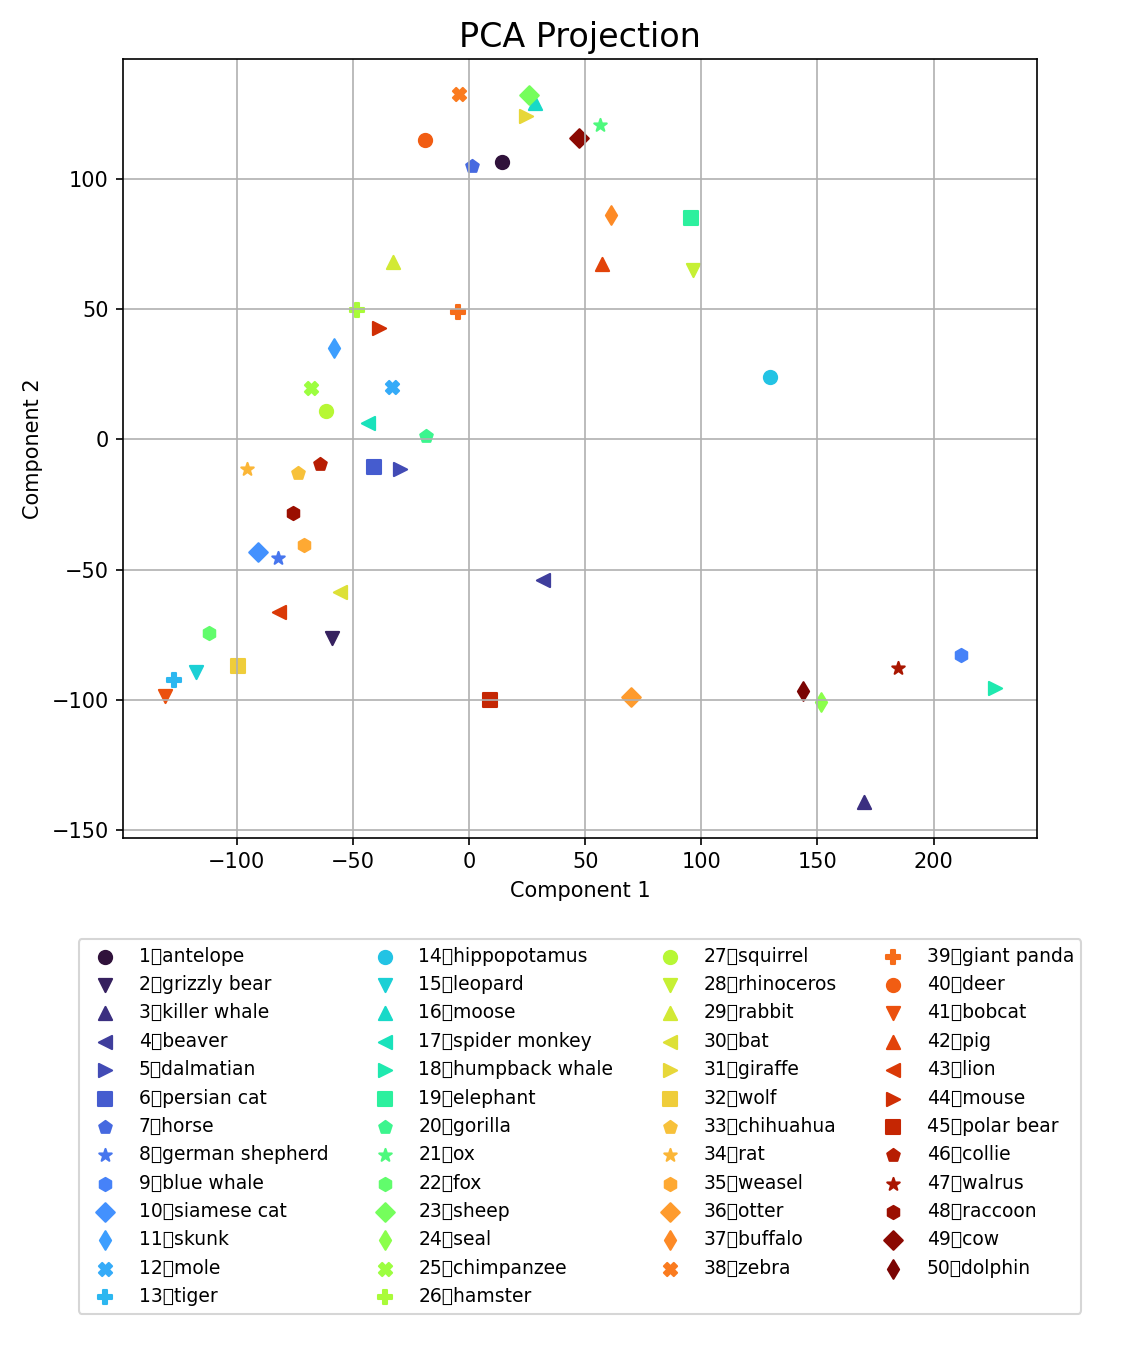
\includegraphics[height=0.75\textheight,width=\textwidth]{pca_projection.png}
  \caption{PCA projection $\mathbb{R}^{85}$ to $\mathbb{R}^{2}$}
\end{figure}
\noindent\rule{\textwidth}{0.4pt}\\

\subsubsection*{Solution 7}
\noindent\rule{\textwidth}{0.4pt}
\subsubsection*{Solution 7 (c)}
\subsubsection*{t-SNE: Perplexity 5}

\begin{figure}[h]
  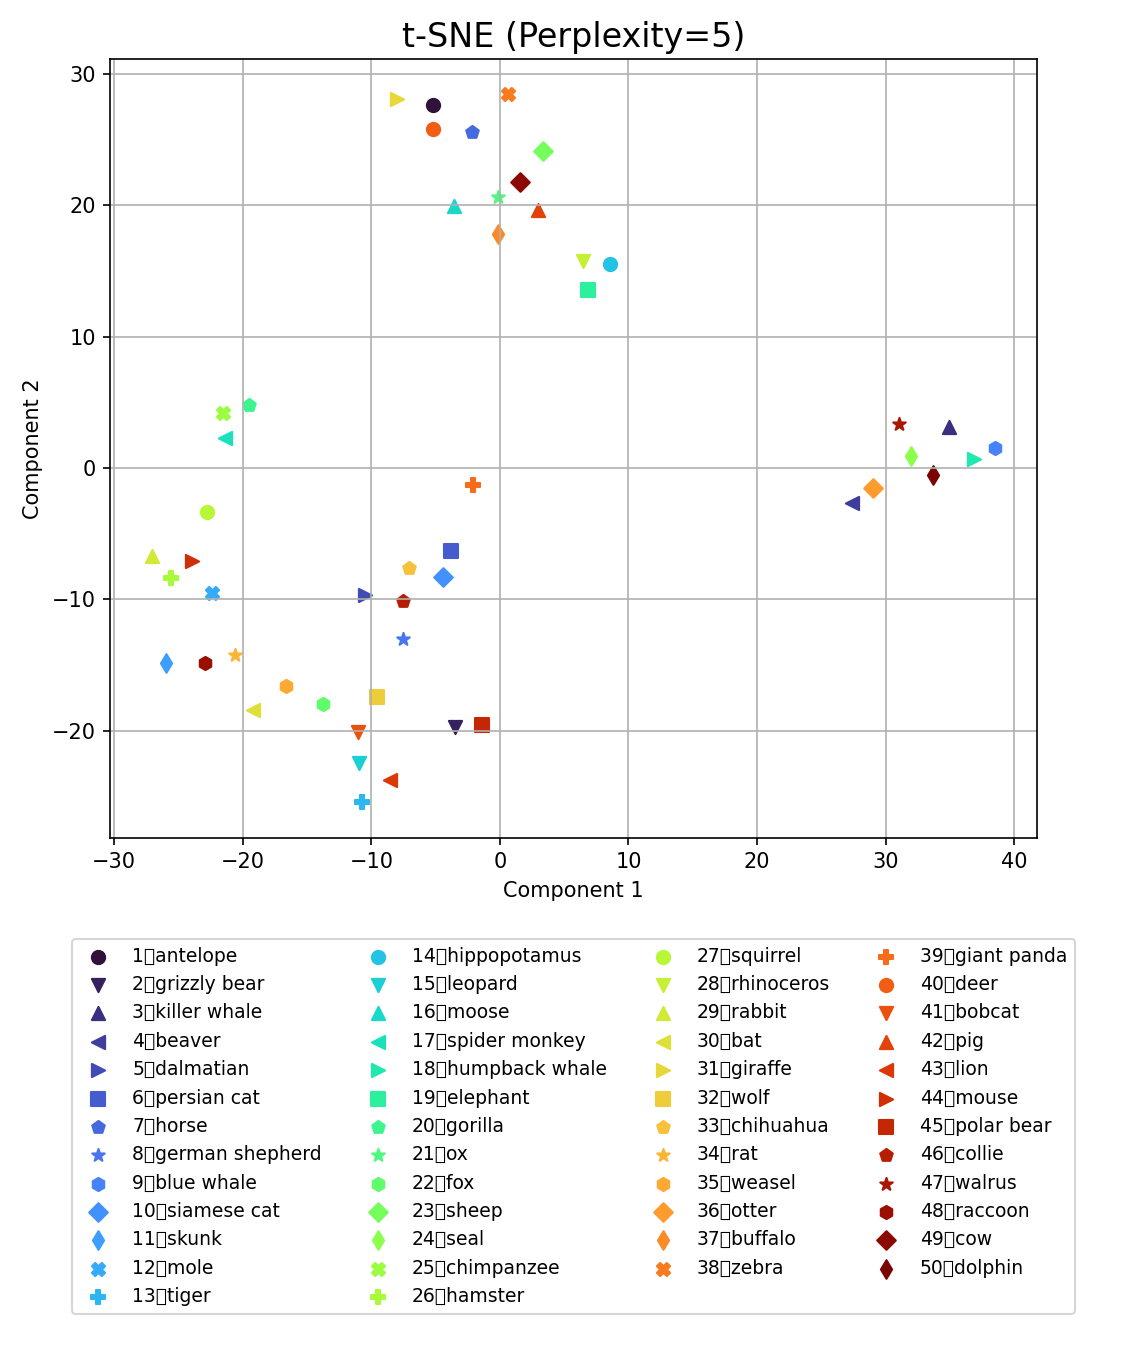
\includegraphics[height=0.75\textheight,width=\textwidth]{t_sne_perplexity5.png}
  \caption{t-SNE plot with perplexity=5}
\end{figure}

\newpage

\subsubsection*{Solution 7}
\noindent\rule{\textwidth}{0.4pt}
\subsubsection*{Solution 7 (c)}
\subsubsection*{t-SNE: Perplexity 10}

\begin{figure}[h]
  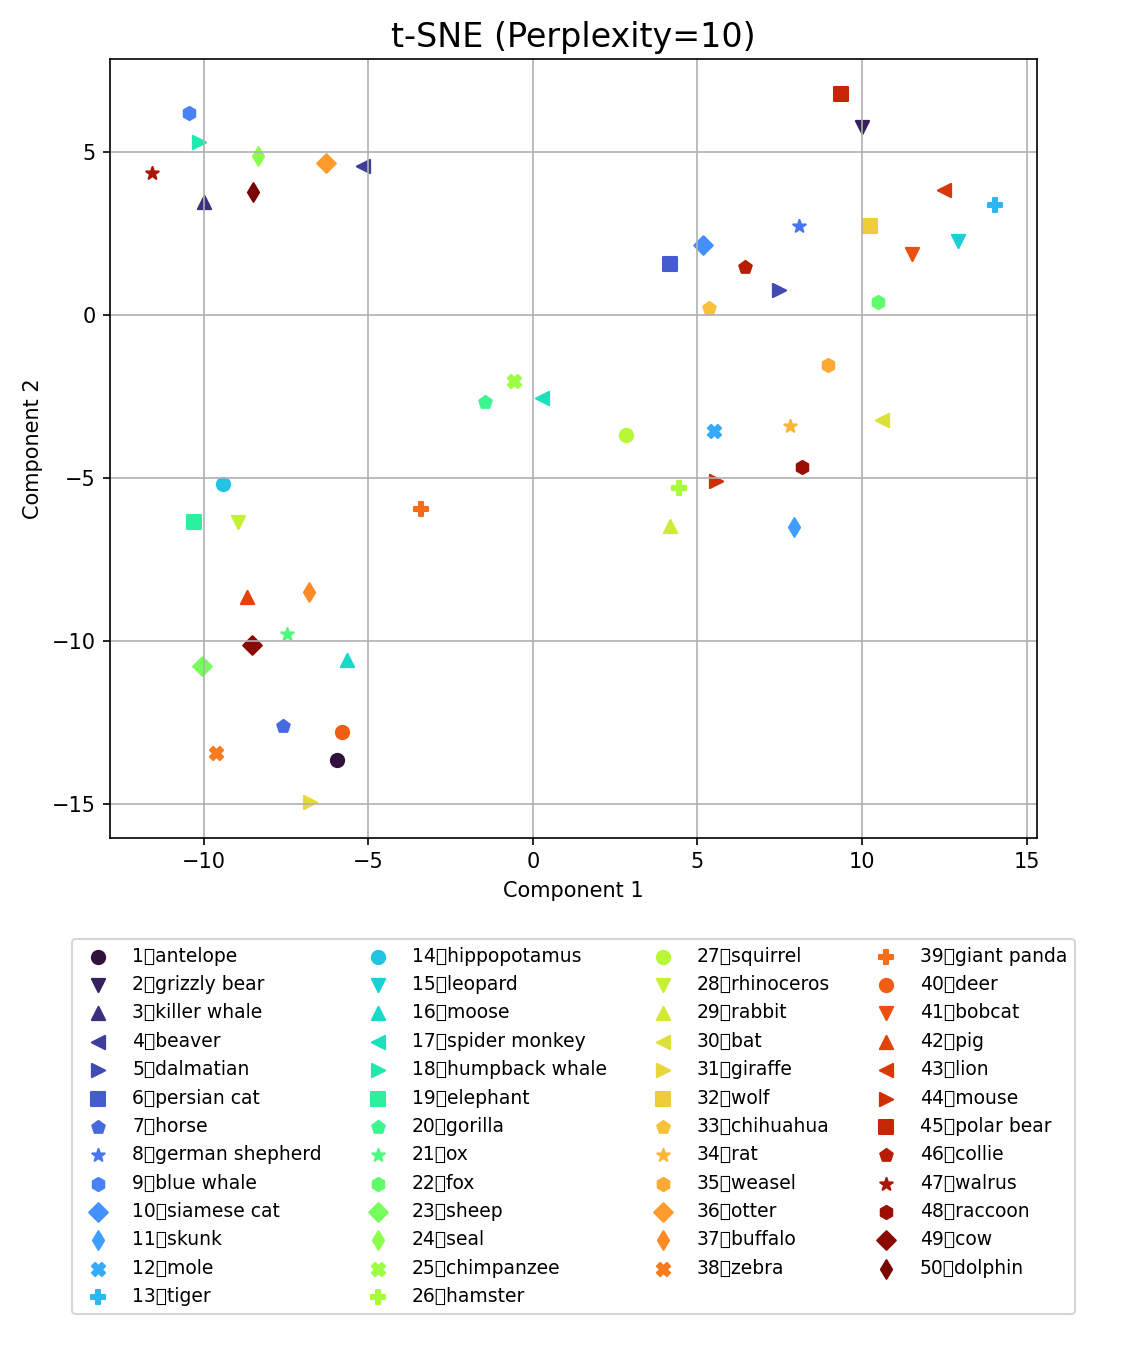
\includegraphics[height=0.75\textheight,width=\textwidth]{t_sne_perplexity10.png}
  \caption{t-SNE plot with perplexity=10}
\end{figure}

\newpage

\subsubsection*{Solution 7}
\noindent\rule{\textwidth}{0.4pt}
\subsubsection*{Solution 7 (c)}
\subsubsection*{t-SNE: Perplexity 25}

\begin{figure}[h]
  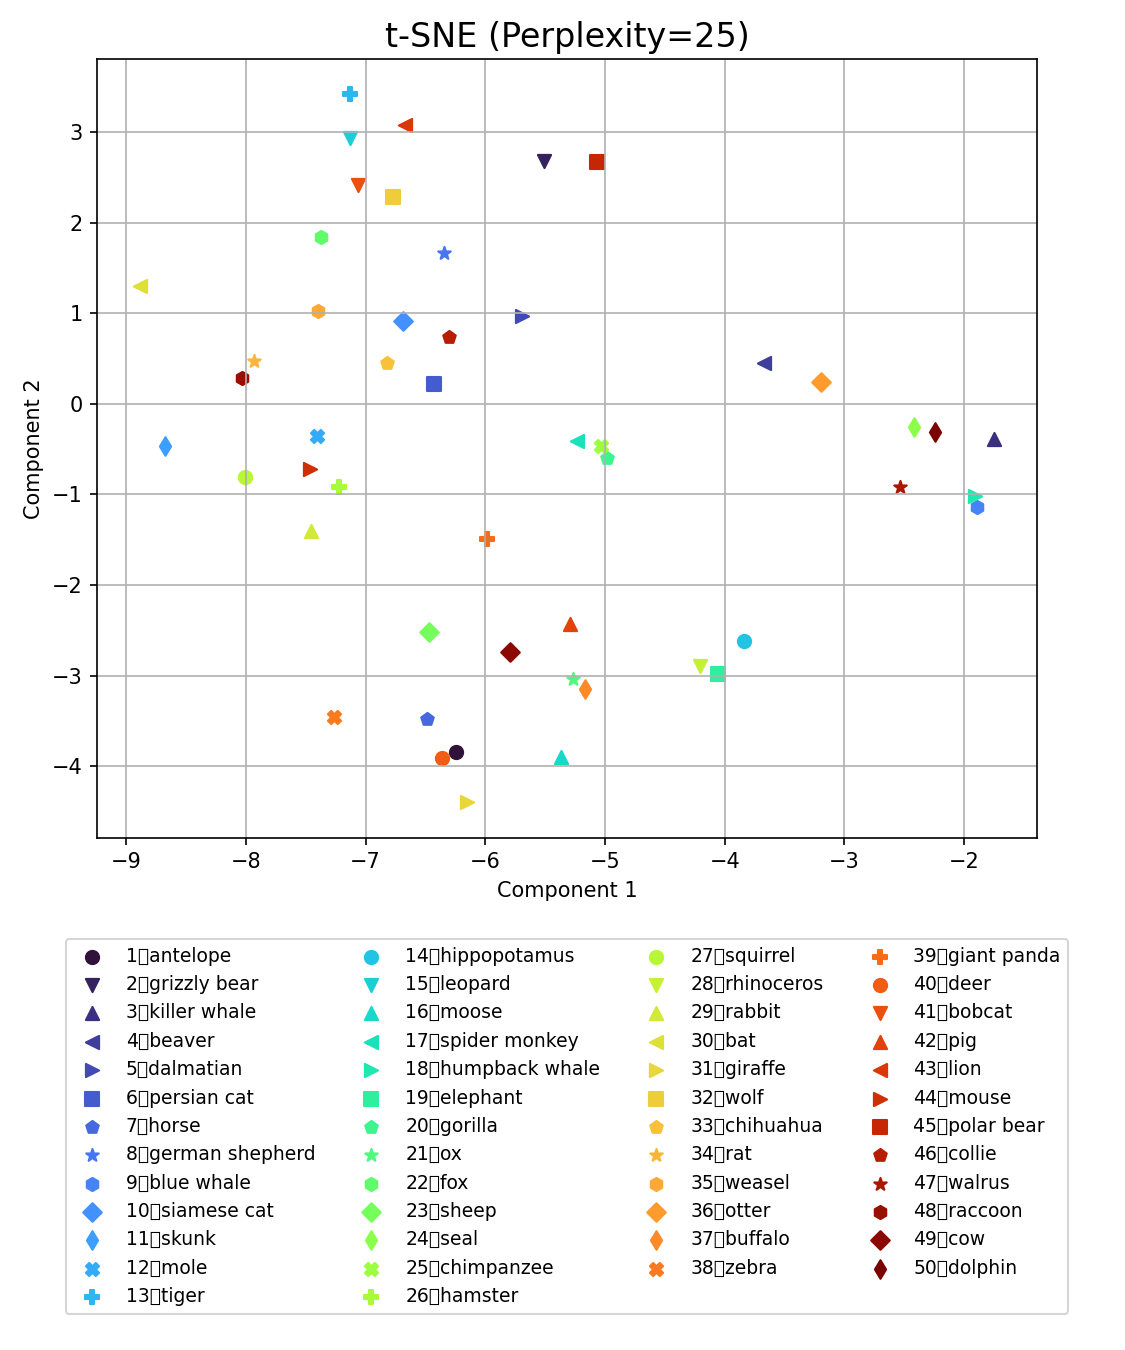
\includegraphics[height=0.75\textheight,width=\textwidth]{t_sne_perplexity25.png}
  \caption{t-SNE plot with perplexity=25}
\end{figure}

\newpage

\subsubsection*{Solution 7}
\noindent\rule{\textwidth}{0.4pt}
\subsubsection*{Solution 7 (c)}
\subsubsection*{t-SNE: Perplexity 49}

\begin{figure}[h]
  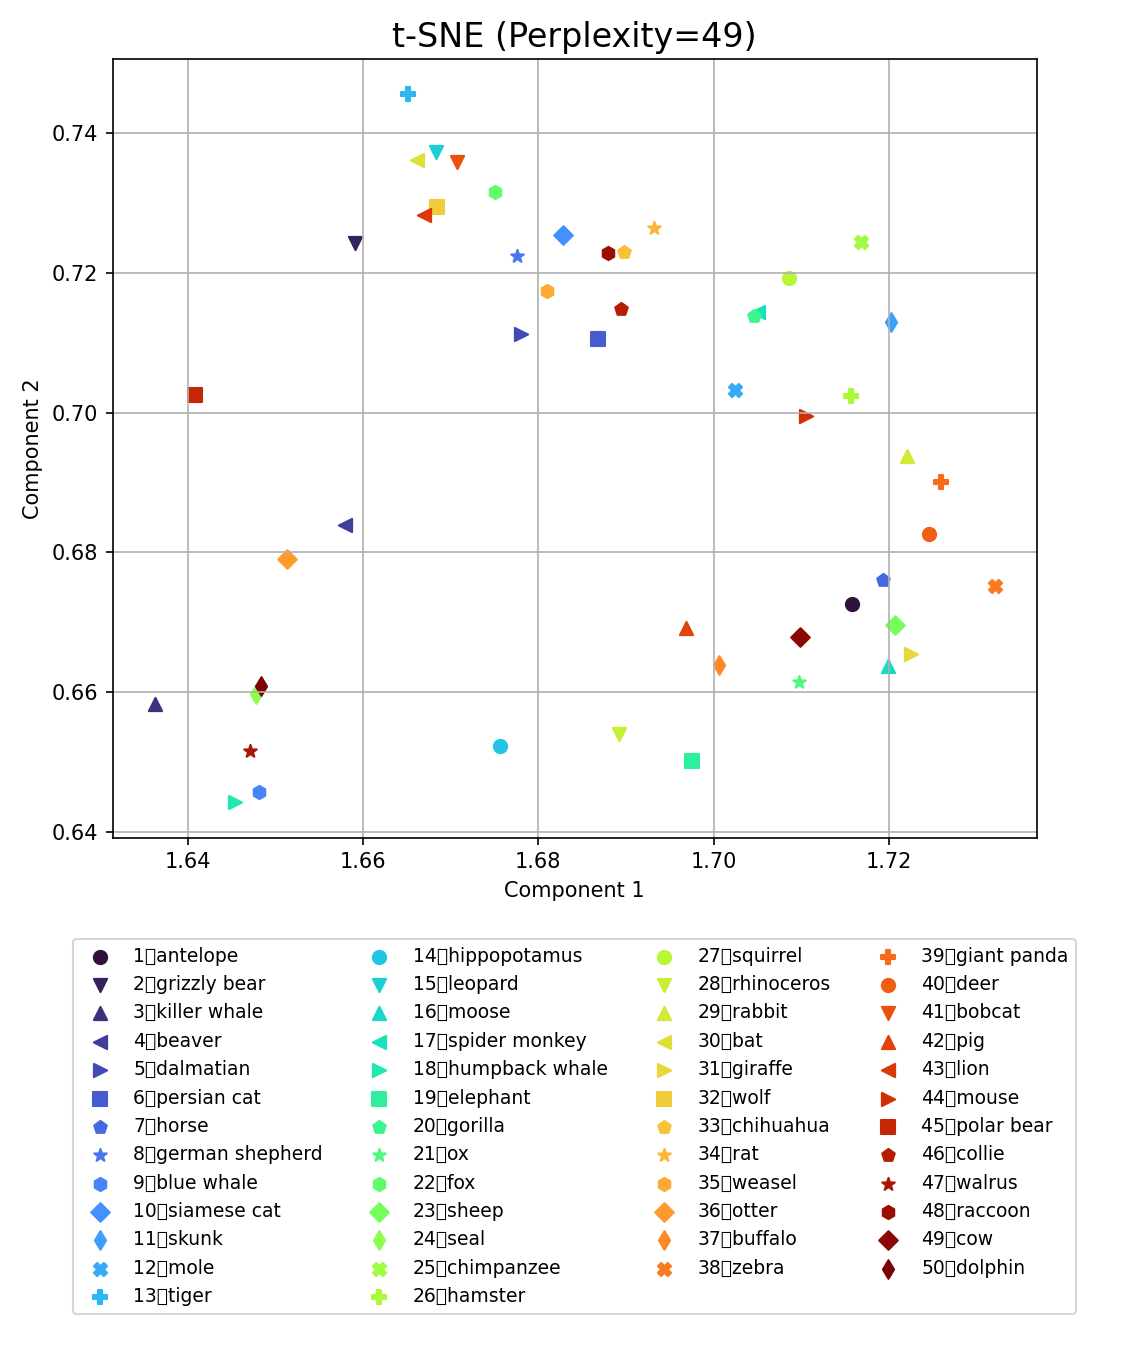
\includegraphics[height=0.75\textheight,width=\textwidth]{t_sne_perplexity49.png}
  \caption{t-SNE plot with perplexity=49. Note: 49 and not 50 because of python indexing starts at 0}
\end{figure}

\newpage

%------------------
% Solution for 8
%------------------
\subsubsection*{Solution 8}
\noindent\rule{\textwidth}{0.4pt}\\
\subsubsection*{Best rank-2 approx to $M$}
Let, \\
\[
M =
\begin{bmatrix}
    1 & 0 & 0 & 0\\
    0 & 0 & 0 & 1\\
    0 & 0 & 1 & 0\\
    0 & 1 & 0 & 0
\end{bmatrix}
\begin{bmatrix}
    4 & 0 & 0 & 0\\
    0 & 3 & 0 & 0\\
    0 & 0 & 2 & 0\\
    0 & 0 & 0 & 1
\end{bmatrix}\begin{bmatrix}
    1 & 0 & 0 & 0 & 0\\
    0 & 1 & 0 & 0 & 0\\
    0 & 0 & 1 & 0 & 0\\
    0 & 0 & 0 & 1 & 0
\end{bmatrix}
\]\\

\begin{flushleft}
The SVD of $M$ is given in the form $M = U \Sigma V^T = \sum_{i=1}^4 \sigma_i u_i v_i^T$.
The best rank-2 approximation, $M_2$, is found by taking the first two terms of the SVD sum, corresponding to the two largest singular values:
\end{flushleft}

$$M_2 = \sigma_1 u_1 v_1^T + \sigma_2 u_2 v_2^T$$

\begin{flushleft}
  From the matrices $U$ (columns $u_i$) and $V^T$ (rows $v_i^T$), we identify the required components:
\end{flushleft}

\[
M =
\underbrace{\begin{bmatrix}
    1 & 0 & 0 & 0\\
    0 & 0 & 0 & 1\\
    0 & 0 & 1 & 0\\
    0 & 1 & 0 & 0
\end{bmatrix}}_{U}
\underbrace{\begin{bmatrix}
    4 & 0 & 0 & 0\\
    0 & 3 & 0 & 0\\
    0 & 0 & 2 & 0\\
    0 & 0 & 0 & 1
\end{bmatrix}}_{\Sigma_{4\times4}}
\underbrace{\begin{bmatrix}
    1 & 0 & 0 & 0 & 0\\
    0 & 1 & 0 & 0 & 0\\
    0 & 0 & 1 & 0 & 0\\
    0 & 0 & 0 & 1 & 0
\end{bmatrix}}_{V^\top}
\]
It follows that:

$$\sigma_1 = 4 \quad u_1 = \begin{bmatrix} 1 \\ 0 \\ 0 \\ 0 \end{bmatrix} \quad v_1^T = \begin{bmatrix} 1 & 0 & 0 & 0 & 0 \end{bmatrix}\quad \sigma_2 = 3 \quad u_2 = \begin{bmatrix} 0 \\ 0 \\ 0 \\ 1 \end{bmatrix} \quad v_2^T = \begin{bmatrix} 0 & 1 & 0 & 0 & 0 \end{bmatrix}$$

\begin{flushleft}
  Now, calculate $M_2$:
\end{flushleft}
 
\begin{align*}
  M_2 &= \sigma_1 u_1 v_1^T + \sigma_2 u_2 v_2^T \\
  &= 4 \left( \begin{bmatrix} 1 \\ 0 \\ 0 \\ 0 \end{bmatrix} \begin{bmatrix} 1 & 0 & 0 & 0 & 0 \end{bmatrix} \right) + 3 \left( \begin{bmatrix} 0 \\ 0 \\ 0 \\ 1 \end{bmatrix} \begin{bmatrix} 0 & 1 & 0 & 0 & 0 \end{bmatrix} \right) \\
    &= 4 \begin{bmatrix}
        1 & 0 & 0 & 0 & 0 \\
        0 & 0 & 0 & 0 & 0 \\
        0 & 0 & 0 & 0 & 0 \\
        0 & 0 & 0 & 0 & 0
        \end{bmatrix} + 3 \begin{bmatrix}
        0 & 0 & 0 & 0 & 0 \\
        0 & 0 & 0 & 0 & 0 \\
        0 & 0 & 0 & 0 & 0 \\
        0 & 1 & 0 & 0 & 0
        \end{bmatrix} 
    = \begin{bmatrix}
        4 & 0 & 0 & 0 & 0 \\
        0 & 0 & 0 & 0 & 0 \\
        0 & 0 & 0 & 0 & 0 \\
        0 & 3 & 0 & 0 & 0
        \end{bmatrix}
\end{align*}

\subsubsection*{\normalfont}{$\therefore$ The best rank-2 approximation to $M$ is:}
\[
M_2 = \begin{bmatrix}
    4 & 0 & 0 & 0 & 0 \\
    0 & 0 & 0 & 0 & 0 \\
    0 & 0 & 0 & 0 & 0 \\
    0 & 3 & 0 & 0 & 0
    \end{bmatrix}
\]

\noindent\rule{\textwidth}{0.4pt}\\

\newpage

%------------------
% Solution for 9 (a)
%------------------
\subsubsection*{Solution 9}
\noindent\rule{\textwidth}{0.4pt}\\
\subsubsection*{Solution 9 (a)}
\subsubsection*{SVD}

\subsubsection*{Python Code}
\begin{lstlisting}
import numpy as np

# set print sig figs
np.set_printoptions(precision=4, suppress=True)

# define matrix M
M = np.array([
    [1, 2, 3],
    [4, 5, 6]
])

# calc "thin" SVD
U, s, Vt = np.linalg.svd(M, full_matrices=False)

# get the first singular value (sigma_1)
sigma_1 = s[0]

# get the first left singular vector (u_1)
u_1 = U[:, 0:1]  

# get the first right singular vector (v_1^T)

v_1_T = Vt[0:1, :] 

# calc rank-1 approximation
M_1 = sigma_1 * (u_1 @ v_1_T)

# print results
print(f"matrix M:\n{M}\n")
print("-" * 30)
print(f"sigma_1 (s[0]): {sigma_1:.4f}\n")
print(f"u_1 (U[:, 0]):\n{u_1}\n")
print(f"v_1^T (Vt[0, :]):\n{v_1_T}\n")
print("-" * 30)
print(f"best rank-1 approximation (M_1):\n{M_1}")
\end{lstlisting}

\newpage

%------------------
% Solution for 9 (a)
%------------------
\subsubsection*{Solution 9}
\noindent\rule{\textwidth}{0.4pt}\\
\subsubsection*{Solution 9 (a)}

\subsubsection*{Compute $M_1$}
\[
M =
\begin{bmatrix}
    1 & 2 & 3 \\
    4 & 5 & 6 
\end{bmatrix}
\]
The best rank-1 approximation $M_1$ is: 
$$M_1 = \sigma_1 u_1 v_1^T$$
\begin{flushleft}
  From the Python output, we have:
\end{flushleft}

$$\sigma_1 \approx 8.7950 \quad u_1 \approx \begin{bmatrix} -0.4042 \\ -0.9147 \end{bmatrix} \quad v_1^T \approx \begin{bmatrix} -0.4287 & -0.5663 & -0.7038 \end{bmatrix}$$

\begin{flushleft}
  Now, calculate $M_1 = \sigma_1 (u_1 v_1^T)$:
\end{flushleft}

\begin{align*}
    M_1 &\approx 8.7950 \left( \begin{bmatrix} -0.4042 \\ -0.9147 \end{bmatrix} \begin{bmatrix} -0.4287 & -0.5663 & -0.7038 \end{bmatrix} \right) \\
    &\approx 8.7950 \begin{bmatrix}
        (-0.4042)(-0.4287) & (-0.4042)(-0.5663) & (-0.4042)(-0.7038) \\
        (-0.9147)(-0.4287) & (-0.9147)(-0.5663) & (-0.9147)(-0.7038)
        \end{bmatrix} \\
    &\approx 8.7950 \begin{bmatrix}
        0.1733 & 0.2289 & 0.2845 \\
        0.3921 & 0.5179 & 0.6438
        \end{bmatrix} \\
    &\approx \begin{bmatrix}
        1.5242 & 2.0131 & 2.5024 \\
        3.4485 & 4.5552 & 5.6621
        \end{bmatrix}
\end{align*}

\subsubsection*{\normalfont}{$\therefore$ The best rank-1 approximation to $M$ is:}
\[
M_1 \approx \begin{bmatrix}
    1.524 & 2.013 & 2.502 \\
    3.449 & 4.555 & 5.662
    \end{bmatrix}
\]


\noindent\rule{\textwidth}{0.4pt}\\

\newpage

%------------------
% Solution for 9 (b)
%------------------
\subsubsection*{Solution 9}
\noindent\rule{\textwidth}{0.4pt}\\
\subsubsection*{Solution 9 (b)}
\subsubsection*{Uniqueness}
Show the decomposition $M = u v^T$ for a rank-1 matrix is not unique.
\begin{flushleft}
Assume $M = u v^T$, where $u \in \mathbb{R}^{p}$ and $v \in \mathbb{R}^{q}$.
Let $c$ be any non-zero scalar (i.e., $c \in \mathbb{R}, c \neq 0$).
Let $a$ and $b$ be vectors such that:
\end{flushleft}

$$a = c u \in \mathbb{R}^{p} \text{ and }b = \left(\frac{1}{c}\right) v \in \mathbb{R}^{q}$$
\begin{flushleft}
If $c \neq 1$, then $a \neq u$ and $b \neq v$. It follows that $(a, b)$ is a different pair of vectors from $(u, v)$.
Next, compute the rank-1 matrix $a b^T$:
\end{flushleft}

\begin{align*}
    a b^T &= (c u) \left( \frac{1}{c} v \right)^T \\
    &= (c u) \left( \frac{1}{c} v^T \right) \\
    &= c \left( \frac{1}{c} \right) (u v^T) \\
    &= 1 \cdot (u v^T) \\
    &= u v^T \\
    &= M
\end{align*}

Hence, $a b^T = u v^T = M$ and $a \neq u$ and $b \neq v$.

\subsubsection*{\normalfont}{$\therefore$ The decomposition is not unique. For any non-zero scalar $c$, the pair $(cu, \frac{1}{c}v)$ will produce the same rank-1 matrix.}

\noindent\rule{\textwidth}{0.4pt}\\

\newpage

\subsubsection*{Code}
\noindent\rule{\textwidth}{0.4pt}
\subsubsection*{Solution 7 Code}
\begin{lstlisting}
import numpy as np
import matplotlib.pyplot as plt
from sklearn.decomposition import PCA
from sklearn.manifold import TSNE
from scipy.spatial.distance import pdist, squareform
import re 

# set plot figure size for better readability 
plt.rcParams['figure.figsize'] = (6, 8)

def load_animal_names(filepath='classes.txt'):
    with open(filepath, 'r') as f:
        names = [line.strip() for line in f.readlines()]
        names = [name.split('.')[-1].replace('+', ' ') for name in names]
    return(names)

def compute_distortion(X_original, Z_embedded):
    # calc pairwise distances for original space (n*(n-1)/2 vector)
    D = pdist(X_original, metric='euclidean')

    # calc pairwise distances for embedded space (n*(n-1)/2 vector)
    D_hat = pdist(Z_embedded, metric='euclidean')
    
    # add a small epsilon to avoid division by zero
    epsilon = 1e-12
    D[D == 0] = epsilon
    D_hat[D_hat == 0] = epsilon
    
    # calc scaling factor c (sum of all pairwise distances)
    c = np.sum(D) / np.sum(D_hat)
    
    # calc scaled embedded distances
    scaled_D_hat = c * D_hat
    
    # calculate distortion for each pair (i, j) with i < j
    Delta_values = np.maximum(D / scaled_D_hat, scaled_D_hat / D)
    
    return(np.mean(Delta_values))

def main():
    # read predicate-matrix-continuous.txt
    X = np.loadtxt('predicate-matrix-continuous.txt')
    # read classes.txt
    animal_names = load_animal_names('classes.txt')
    
    # initalize list to hold embeddings and their titles
    embeddings_to_plot = []

    # pca model
    pca = PCA(n_components=2, random_state=42)
    Z_pca = pca.fit_transform(X)
    embeddings_to_plot.append(('PCA Projection', Z_pca))

    # note: 49 ~ 50 its just python indexing
    perplexities = [5, 10, 25, 49]
    for p in perplexities:
        print(f"Running t-SNE with perplexity={p}...")
        tsne = TSNE(n_components=2, perplexity=p, random_state=42, 
                    init='pca', learning_rate='auto')
        Z_tsne = tsne.fit_transform(X)
        embeddings_to_plot.append((f't-SNE (Perplexity={p})', Z_tsne))
    
    for title, Z in embeddings_to_plot:
        # set plt configs
        fig = plt.figure(figsize=(7.5, 9))
        grid_shape = (3, 3)
        ax_plot = plt.subplot2grid(grid_shape, (0, 0), rowspan=2, colspan=3)
        ax_legend = plt.subplot2grid(grid_shape, (2, 0), rowspan=1, colspan=3)
        
        # plot data
        for j, name in enumerate(animal_names):
            color = colors[j]
            marker = markers[j % len(markers)]
            
            ax_plot.scatter(Z[j, 0], Z[j, 1], 
                            color=color, 
                            marker=marker, 
                            label=name, 
                            s=40) # s=40 is a reasonable marker size
        
        ax_plot.set_title(title, fontsize=16)
        ax_plot.set_xlabel('Component 1')
        ax_plot.set_ylabel('Component 2')
        ax_plot.grid(True)
        
        # set legend settings
        handles, labels = ax_plot.get_legend_handles_labels()
        ax_legend.axis('off')
        ax_legend.legend(handles, labels, loc='center', ncol=4, fontsize=9)
        
        # save plot
        # Use tight_layout to ensure no overlap
        plt.tight_layout()
        clean_title = title.lower()
        clean_title = re.sub(r'[^\w\s-]', '', clean_title) 
        clean_title = re.sub(r'[\s-]+', '_', clean_title).strip('_')
        filename = f"{clean_title}.png"
        
        plt.savefig(filename, dpi=150) # 150 dpi is good for print
        plt.close(fig) # Close the figure to free memory

    # calc distortion
    distortions = {}
    
    # store all embeddings in a dict for distortion calculation
    all_embeddings_dict = {title: Z for title, Z in embeddings_to_plot}
        
    for key, Z in all_embeddings_dict.items():
        distortion = compute_distortion(X, Z)
        distortions[key] = distortion
        print(f"{key} average distortion: {distortion:.4f}")
        
    best_embedding = min(distortions, key=distortions.get)
    min_distortion = distortions[best_embedding]
    
    print(f"lowest average distortion is: {best_embedding}")
    print(f"minimum distortion: {min_distortion:.4f}")

\end{lstlisting}

\newpage

\subsubsection*{Code}
\noindent\rule{\textwidth}{0.4pt}
\subsubsection*{Solution 9 Code}
\begin{lstlisting}
import numpy as np

# set print sig figs
np.set_printoptions(precision=4, suppress=True)

# define matrix M
M = np.array([
    [1, 2, 3],
    [4, 5, 6]
])

# calc "thin" SVD
U, s, Vt = np.linalg.svd(M, full_matrices=False)

# get the first singular value (sigma_1)
sigma_1 = s[0]

# get the first left singular vector (u_1)
u_1 = U[:, 0:1]  

# get the first right singular vector (v_1^T)

v_1_T = Vt[0:1, :] 

# calc rank-1 approximation
M_1 = sigma_1 * (u_1 @ v_1_T)

# print results
print(f"matrix M:\n{M}\n")
print("-" * 30)
print(f"sigma_1 (s[0]): {sigma_1:.4f}\n")
print(f"u_1 (U[:, 0]):\n{u_1}\n")
print(f"v_1^T (Vt[0, :]):\n{v_1_T}\n")
print("-" * 30)
print(f"best rank-1 approximation (M_1):\n{M_1}")
\end{lstlisting}

\noindent\rule{\textwidth}{0.4pt}

\end{document}

\begin{comment}
%------------------
% Solution for 2(a),2(b), and 2(c)
%------------------
\subsection*{Solution 2}
\noindent\rule{\textwidth}{0.4pt}\\
\subsubsection*{Solution 2 (a)}
\subsubsection*{Step 1: Define Euclidean distance ($\ell_2$)}
\parbox{\textwidth}{

$$\ell_2 = \|p - q\|_2 = \sqrt{\sum_{i=1}^{n} (p_i - q_i)^2}$$

}

\subsubsection*{Step 2: Compute $\ell_2$}
\parbox{\textwidth}{
Let $p=1$ and $q=10$
$$
\begin{aligned}
\ell_2 &= \sqrt{\sum_{i=1}^{n} (p_i - q_i)^2}\\
\ell_2 &= \sqrt{\sum_{i=1}^{1} (1 - 10)^2}\\
\ell_2 &= \sqrt{(- 9)^2}\\
\ell_2 &= 9
\end{aligned}
$$
}
\subsubsection*{\normalfont}{$\therefore$ $\ell_{2} = 9$}

\noindent\rule{\textwidth}{0.4pt}\\

\subsubsection*{Solution 2 (b)}
\subsubsection*{Step 1: Define Euclidean distance ($\ell_2$)}
\parbox{\textwidth}{

$$\ell_2 = \|p - q\|_2 = \sqrt{\sum_{i=1}^{n} (p_i - q_i)^2}$$

}

\subsubsection*{Step 2: Compute $\ell_2$}
\parbox{\textwidth}{
Let $p = \begin{bmatrix} -1 \\ 12 \end{bmatrix}, q = \begin{bmatrix} 6 \\ -12 \end{bmatrix}$
$$
\begin{aligned}
\ell_2 &= \sqrt{\sum_{i=1}^{n} (p_i - q_i)^2}\\
\ell_2 &= \sqrt{(p_1 - q_1)^{2}+(p_2 - q_2)^{2}}\\
\ell_2 &= \sqrt{(-1 - 6)^{2}+(12 - (-12))^{2}}\\
\ell_2 &= \sqrt{(-7)^{2}+(24)^{2}}\\
\ell_2 &= \sqrt{625}\\
\ell_2 &= 25
\end{aligned}
$$
}
\subsubsection*{\normalfont}{$\therefore$ $\ell_{2} = 25$}

\noindent\rule{\textwidth}{0.4pt}\\


\subsection*{Solution 2}
\noindent\rule{\textwidth}{0.4pt}\\
\subsubsection*{Solution 2 (c)}
\subsubsection*{Step 1: Define Euclidean distance ($\ell_2$)}
\parbox{\textwidth}{

$$\ell_2 = \|p - q\|_2 = \sqrt{\sum_{i=1}^{n} (p_i - q_i)^2}$$

}

\subsubsection*{Step 2: Compute $\ell_2$}
\parbox{\textwidth}{
Let $p = \begin{bmatrix} 1 \\ 5 \\ -1 \end{bmatrix}, q = \begin{bmatrix} 5 \\ 2 \\ 11 \end{bmatrix}$
$$
\begin{aligned}
\ell_2 &= \sqrt{\sum_{i=1}^{n} (p_i - q_i)^2}\\
\ell_2 &= \sqrt{(p_1 - q_1)^{2}+(p_2 - q_2)^{2}+(p_3 - q_3)^{2}}\\
\ell_2 &= \sqrt{(1 - 5)^{2}+(5 - 2)^{2}+(-1 - 11)^{2}}\\
\ell_2 &= \sqrt{(-4)^{2}+(3)^{2}+(-12)^{2}}\\
\ell_2 &= \sqrt{169}\\
\ell_2 &= 13
\end{aligned}
$$
}
\subsubsection*{\normalfont}{$\therefore$ $\ell_{2} = 13$}

\noindent\rule{\textwidth}{0.4pt}\\

\newpage

%------------------
% Solution for 3(a) and 3(b)
%------------------
\subsection*{Solution 3}
\noindent\rule{\textwidth}{0.4pt}\\
\subsubsection*{Solution 3 (a)}
\subsubsection*{Step 1: Normalize the vector $x$}
\parbox{\textwidth}{
Let $x = \begin{bmatrix} 10 \\ 15 \\ 25 \end{bmatrix}$

$$\sum_{i=1}^{3} x_{i} = x_{1} + x_{2} + x_{3} = 10 + 15 + 25 = 50$$

Now, divide each entry by the total sum:\\

$$p = \frac{1}{50} \cdot x = \frac{1}{50} \begin{bmatrix} 10 \\ 15 \\ 25 \end{bmatrix} = \begin{bmatrix} 10/50 \\ 15/50 \\ 25/50 \end{bmatrix} = \begin{bmatrix} 0.2 \\ 0.3 \\ 0.5 \end{bmatrix}$$
}
\subsubsection*{\normalfont}{$\therefore$ the result ($p$) of scaling vertor $x$ is the following:}
$$p = \begin{bmatrix} 0.2 \\ 0.3 \\ 0.5 \end{bmatrix}$$ \\

\noindent\rule{\textwidth}{0.4pt}\\

\subsubsection*{Solution 3 (b)}
\subsubsection*{Step 1: Define dimension of the probability simplex}
\parbox{\textwidth}{
The dimension of vector $p$ is $3$ and $k=n-1$ where $k$ is the dimension of the probability simplex
}
\subsubsection*{\normalfont}{$\therefore$ vector $p$ lies in the probability simplex($\Delta_2$) for $k=2$}

\noindent\rule{\textwidth}{0.4pt}\\

\newpage

%------------------
% Solution for 4
%------------------
\subsection*{Solution 4}
\noindent\rule{\textwidth}{0.4pt}\\

\subsubsection*{Step 1: Define probability simplex $\Delta_2$ }
\parbox{\textwidth}{

For a point to be scalable to $\Delta_2$, after scaling it must satisfy:
\begin{itemize}
\item All components must be non-negative
\item The sum of components must equal 1
\end{itemize}
}

\subsubsection*{Step 2: Give example that violates one of the rules in Step 1}
\parbox{\textwidth}{
Let $x = \begin{bmatrix} 1 \\ -2 \end{bmatrix}$

The second component of $x$ violates the first rule, all components for a point must be non-negative $\Delta_2$.
}

\subsubsection*{\normalfont}{$\therefore$ the point $x = \begin{bmatrix} 1 \\ -2 \end{bmatrix}$ cannot be scaled to lie in $\Delta_{2}$}

\noindent\rule{\textwidth}{0.4pt}\\

\newpage

%------------------
% Solution for 5
%------------------
\subsection*{Solution 5}
\noindent\rule{\textwidth}{0.4pt}\\

\subsubsection*{Visualizing the Simplex $\Delta_3$ in 2D Projections}
\parbox{\textwidth}{
Here are the three 2D views of the probability simplex $\Delta_3$. Each plot is a \textit{shadow} of the 3D triangle, viewed along one of the principal axes.
}

%---------------------------------------------------
%  FIGURE 1: x1 vs x2 Projection
%---------------------------------------------------
\begin{figure}[h!]
\centering
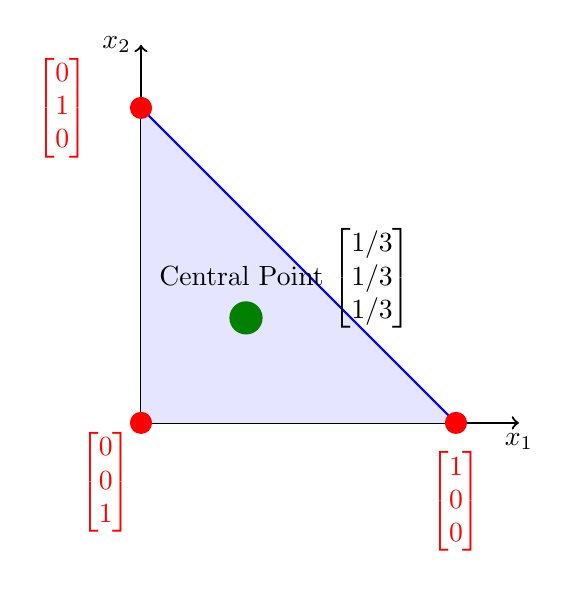
\begin{tikzpicture}[scale=4]
    % Axes
    \draw[->, thick] (0,0) -- (1.2,0) node[below] {$x_1$};
    \draw[->, thick] (0,0) -- (0,1.2) node[left] {$x_2$};

    % The projected simplex region (x1 + x2 <= 1)
    \fill[blue!10] (0,0) -- (1,0) -- (0,1) -- cycle;
    \draw[blue, thick] (1,0) -- (0,1);

    % The three vertices of the simplex
    \fill[red] (1,0) circle (1pt) node[shift={(0, -1)}] {$\begin{bmatrix} 1 \\ 0 \\ 0 \end{bmatrix}$};
    \fill[red] (0,1) circle (1pt) node[shift={(-1, 0)}] {$\begin{bmatrix} 0 \\ 1 \\ 0 \end{bmatrix}$};
    \fill[red] (0,0) circle (1pt) node[below left] {$\begin{bmatrix} 0 \\ 0 \\ 1 \end{bmatrix}$};

    % The central point (centroid)
    \fill[green!50!black] (1/3, 1/3) circle (1.5pt) node[shift={(0.5,0.5)}, black] {Central Point $\begin{bmatrix} 1/3 \\ 1/3 \\ 1/3 \end{bmatrix}$};
\end{tikzpicture}
\caption{View 1: Projection onto the $x_1$-$x_2$ plane.}
\label{fig:x1x2}
\end{figure}

%---------------------------------------------------
%  FIGURE 2: x2 vs x3 Projection
%---------------------------------------------------
\begin{figure}[h!]
\centering
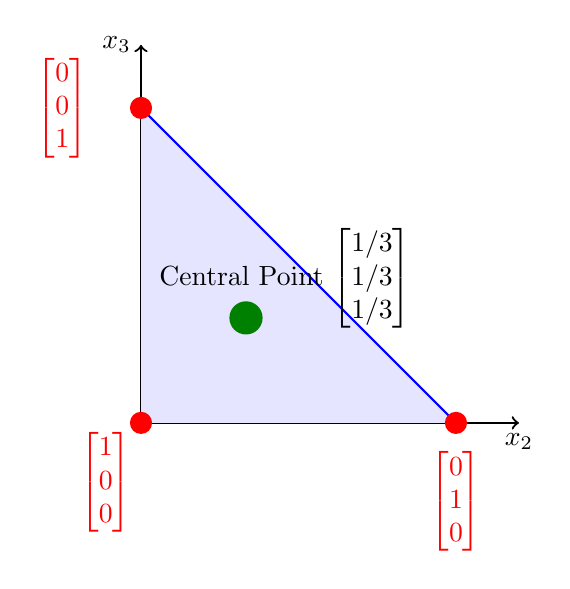
\begin{tikzpicture}[scale=4]
    % Axes
    \draw[->, thick] (0,0) -- (1.2,0) node[below] {$x_2$};
    \draw[->, thick] (0,0) -- (0,1.2) node[left] {$x_3$};

    % The projected simplex region (x2 + x3 <= 1)
    \fill[blue!10] (0,0) -- (1,0) -- (0,1) -- cycle;
    \draw[blue, thick] (1,0) -- (0,1);

    % The three vertices of the simplex
    \fill[red] (1,0) circle (1pt) node[shift={(0, -1)}] {$\begin{bmatrix} 0 \\ 1 \\ 0 \end{bmatrix}$};
    \fill[red] (0,1) circle (1pt) node[shift={(-1, 0)}] {$\begin{bmatrix} 0 \\ 0 \\ 1 \end{bmatrix}$};
    \fill[red] (0,0) circle (1pt) node[below left] {$\begin{bmatrix} 1 \\ 0 \\ 0 \end{bmatrix}$};

    % The central point (centroid)
    \fill[green!50!black] (1/3, 1/3) circle (1.5pt) node[shift={(0.5,0.5)}, black] {Central Point $\begin{bmatrix} 1/3 \\ 1/3 \\ 1/3 \end{bmatrix}$};
\end{tikzpicture}
\caption{View 2: Projection onto the $x_2$-$x_3$ plane.}
\label{fig:x2x3}
\end{figure}

\newpage

\subsection*{Solution 5}
\noindent\rule{\textwidth}{0.4pt}\\
%---------------------------------------------------
%  FIGURE 3: x1 vs x3 Projection
%---------------------------------------------------
\begin{figure}[h!]
\centering
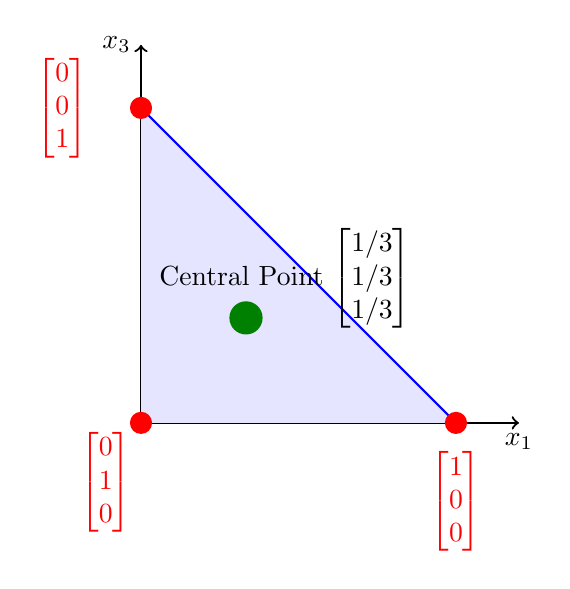
\begin{tikzpicture}[scale=4]
    % Axes
    \draw[->, thick] (0,0) -- (1.2,0) node[below] {$x_1$};
    \draw[->, thick] (0,0) -- (0,1.2) node[left] {$x_3$};

    % The projected simplex region (x1 + x3 <= 1)
    \fill[blue!10] (0,0) -- (1,0) -- (0,1) -- cycle;
    \draw[blue, thick] (1,0) -- (0,1);

    % The three vertices of the simplex
    \fill[red] (1,0) circle (1pt) node[shift={(0, -1)}] {$\begin{bmatrix} 1 \\ 0 \\ 0 \end{bmatrix}$};
    \fill[red] (0,1) circle (1pt) node[shift={(-1, 0)}] {$\begin{bmatrix} 0 \\ 0 \\ 1 \end{bmatrix}$};
    \fill[red] (0,0) circle (1pt) node[below left] {$\begin{bmatrix} 0 \\ 1 \\ 0 \end{bmatrix}$};

    % The central point (centroid)
    \fill[green!50!black] (1/3, 1/3) circle (1.5pt) node[shift={(0.5,0.5)}, black] {Central Point $\begin{bmatrix} 1/3 \\ 1/3 \\ 1/3 \end{bmatrix}$};
\end{tikzpicture}
\caption{View 3: Projection onto the $x_1$-$x_3$ plane.}
\label{fig:x1x3}
\end{figure}

\noindent\rule{\textwidth}{0.4pt}\\

\newpage

%------------------
% Solution for 6
%------------------
\subsection*{Solution 6}
\noindent\rule{\textwidth}{0.4pt}\\

\subsubsection*{6 (a): $\ell_1$ for $p$ and $q$}

\parbox{\textwidth}{The $\ell_1$ distance between two vectors $p, q \in \mathbb{R}^n$ is given by:
$$\|p-q\|_1 = \sum_{i=1}^n |p_i - q_i|$$

Let $p = \begin{bmatrix} 1/2 \\ 1/4 \\ 1/8 \\ 1/8 \end{bmatrix}$ and $q = \begin{bmatrix} 1/4 \\ 1/4 \\ 1/4 \\ 1/4 \end{bmatrix}$

\begin{align*}
    \|p-q\|_1 &= \left|\frac{1}{2} - \frac{1}{4}\right| + \left|\frac{1}{4} - \frac{1}{4}\right| + \left|\frac{1}{8} - \frac{1}{4}\right| + \left|\frac{1}{8} - \frac{1}{4}\right| \\
    &= \left|\frac{2}{4} - \frac{1}{4}\right| + |0| + \left|\frac{1}{8} - \frac{2}{8}\right| + \left|\frac{1}{8} - \frac{2}{8}\right| \\
    &= \frac{1}{4} + 0 + \left|-\frac{1}{8}\right| + \left|-\frac{1}{8}\right| \\
    &= \frac{1}{4} + \frac{1}{8} + \frac{1}{8} = \frac{2}{8} + \frac{1}{8} + \frac{1}{8} = \frac{4}{8} = \frac{1}{2}
\end{align*}
}
\subsubsection*{\normalfont}{$\therefore$ $\ell_{1}= \frac{1}{2}$}

\noindent\rule{\textwidth}{0.4pt}\\

\newpage

\subsection*{Solution 6}
\noindent\rule{\textwidth}{0.4pt}\\

\subsubsection*{6 (b): $\ell_1$ for $q$ and $r$}
\parbox{\textwidth}{The $\ell_1$ distance between two vectors $q, r \in \mathbb{R}^n$ is given by:
$$\|q-r\|_1 = \sum_{i=1}^n |q_i - r_i|$$

Let $q = \begin{bmatrix} 1/4 \\ 1/4 \\ 1/4 \\ 1/4 \end{bmatrix}$ and $r = \begin{bmatrix} 1/2 \\ 0 \\ 1/4 \\ 1/4 \end{bmatrix}$

\begin{align*}
\|q-r\|_1 &= \sum_{i=1}^{4} |q_i - r_i| \\
&= \left|\frac{1}{4} - \frac{1}{2}\right| + \left|\frac{1}{4} - 0\right| + \left|\frac{1}{4} - \frac{1}{4}\right| + \left|\frac{1}{4} - \frac{1}{4}\right| \\
&= \left|\frac{1}{4} - \frac{2}{4}\right| + \left|\frac{1}{4}\right| + |0| + |0| \\
&= \left|-\frac{1}{4}\right| + \frac{1}{4} + 0 + 0 \\
&= \frac{1}{4} + \frac{1}{4} \\
&= \frac{1}{2}
\end{align*}
}

\subsubsection*{\normalfont}{$\therefore$ $\ell_1 = \frac{1}{2}$}

\noindent\rule{\textwidth}{0.4pt}\\

\newpage

\subsection*{Solution 6}
\noindent\rule{\textwidth}{0.4pt}\\

\subsubsection*{6 (c): KL divergence $K(p, q)$}
\parbox{\textwidth}{
The Kullback-Leibler (KL) divergence from a distribution $p$ to a distribution $q$ is defined as:
$$K(p, q) = \sum_{i} p_i \ln \frac{p_i}{q_i}$$
Let $p = \begin{bmatrix} 1/2 \\ 1/4 \\ 1/8 \\ 1/8 \end{bmatrix}$ and $q = \begin{bmatrix} 1/4 \\ 1/4 \\ 1/4 \\ 1/4 \end{bmatrix}$
}

\begin{align*}
K(p, q) &= \sum_{i=1}^{4} p_i \ln\left(\frac{p_i}{q_i}\right) \\
&= p_1 \ln\left(\frac{p_1}{q_1}\right) + p_2 \ln\left(\frac{p_2}{q_2}\right) + p_3 \ln\left(\frac{p_3}{q_3}\right) + p_4 \ln\left(\frac{p_4}{q_4}\right) \\
&= \frac{1}{2}\ln\left(\frac{1/2}{1/4}\right) + \frac{1}{4}\ln\left(\frac{1/4}{1/4}\right) + \frac{1}{8}\ln\left(\frac{1/8}{1/4}\right) + \frac{1}{8}\ln\left(\frac{1/8}{1/4}\right) \\
&= \frac{1}{2}\ln(2) + \frac{1}{4}\ln(1) + \frac{1}{8}\ln\left(\frac{1}{2}\right) + \frac{1}{8}\ln\left(\frac{1}{2}\right) \\
&= \frac{1}{2}\ln(2) + \frac{1}{4}(0) - \frac{1}{8}\ln(2) - \frac{1}{8}\ln(2) \\
&= \frac{1}{2}\ln(2) - \frac{2}{8}\ln(2) \\
&= \left(\frac{1}{2} - \frac{1}{4}\right)\ln(2) \\
&= \frac{1}{4}\ln(2)
\end{align*}

\subsubsection*{\normalfont{$\therefore$ $K(p,q) = \frac{1}{4}\ln(2)$}}
\noindent\rule{\textwidth}{0.4pt}\\

\newpage

\subsection*{Solution 6}
\noindent\rule{\textwidth}{0.4pt}\\

\subsubsection*{6 (d): KL divergence $K(q, r)$}
\parbox{\textwidth}{
The Kullback-Leibler (KL) divergence from a distribution $q$ to a distribution $r$ is defined as:
$$K(q, r) = \sum_{i} q_i \ln \frac{q_i}{r_i}$$
Let $q = \begin{bmatrix} 1/4 \\ 1/4 \\ 1/4 \\ 1/4 \end{bmatrix}$ and $r = \begin{bmatrix} 1/2 \\ 0 \\ 1/4 \\ 1/4 \end{bmatrix}$ \\

Looking at the second component ($i=2$). Here, $q_2 = \frac{1}{4} > 0$ while $r_2 = 0$. The corresponding term in the KL divergence sum, $q_2 \ln\left(\frac{q_2}{r_2}\right)$, involves division by zero. \\

Hence, the divergence will be infinite.
}
\subsubsection*{\normalfont}{$\therefore$ $K(q, r) = \infty$}

\noindent\rule{\textwidth}{0.4pt}\\

\newpage
%------------------
% Solution for 7
%------------------
\subsection*{Solution 7}
\noindent\rule{\textwidth}{0.4pt}\\

\subsubsection*{Python Code}
\begin{lstlisting}
import numpy as np
import matplotlib.pyplot as plt
from extract_feature import compute_or_load_features
from sklearn.neighbors import KNeighborsClassifier

def run_nearest_neighbor(x_train, y_train, x_test, y_test):
    # create classifier    
    nn_classifier = KNeighborsClassifier(n_neighbors=1, algorithm='auto')

    # train 
    nn_classifier.fit(x_train, y_train)

    # test and report accuracy
    test_acc = nn_classifier.score(x_test, y_test)

    print("Nearest neighbor accuracy on the test set: %f"%test_acc)

    return nn_classifier


def analyze_nn(classifier, x_train, y_train, x_test, y_test, x_test_features, N, model_type):
    """
    generalization to grab indices, predictions, and make plots
    """
    # list of image labels
    CIFAR_CLASSES = ['airplane', 'automobile', 'bird', 'cat', 'deer', 'dog', 'frog', 'horse', 'ship', 'truck']

    # get predictions of classifier on test data
    y_pred = classifier.predict(x_test_features)
    
    # define bool condtion where classifier made correct prediction
    is_correct = (y_pred == y_test)
    
    # get indices for correct and incorrect samples
    correct_indices_test = np.where(is_correct)[0][:N]
    incorrect_indices_test = np.where(~is_correct)[0][:N]
    
    # make image plots 
    def plot_pairs(title, test_indices):
        
        # check just in case of bad result.. nema nista
        if len(test_indices) == 0:
            return
            
        # Get the feature vectors for the selected test images (flattened)
        selected_test_features = x_test_features[test_indices]
        
        # get nearest neighbor
        # note: kneighbors -> (distances, indices).. only need the indices.
        _, nn_train_indices_2D = classifier.kneighbors(X=selected_test_features, n_neighbors=1)
        
        # 2D -> 1D
        nn_train_indices = nn_train_indices_2D.flatten()
        
        # get images and labels for the selected test points
        test_images_sample = x_test[test_indices]
        test_labels_sample = y_test[test_indices]
        
        #get the RAW neighbor image and label from the training points
        nn_images_sample = x_train[nn_train_indices]
        nn_labels_sample = y_train[nn_train_indices]
        
        # prediction is nearest neighbor label
        y_pred_sample = nn_labels_sample
        
        # reshape (N, C, H, W) to (N, H, W, C) for plot
        test_images_plt = test_images_sample.transpose(0, 2, 3, 1)
        nn_images_plt = nn_images_sample.transpose(0, 2, 3, 1)

        N_plot = len(test_indices)
        
        # just in case only 1 image is plotted (axes will be 1D instead of 2D)
        if N_plot == 1:
            fig, axes = plt.subplots(N_plot, 2, figsize=(6, 2))
            axes = axes[np.newaxis, :] 
        else:
            fig, axes = plt.subplots(N_plot, 2, figsize=(6, 2 * N_plot))
            
        fig.suptitle(title, fontsize=14, y=1.02)
        
        for i in range(N_plot):
            is_correct = (test_labels_sample[i] == y_pred_sample[i])
            pred_color = 'green' if is_correct else 'red'
            
            # plot test image
            axes[i, 0].imshow(test_images_plt[i] / 255.0)
            axes[i, 0].set_title(f"Test ({CIFAR_CLASSES[test_labels_sample[i]]})", fontsize=10)
            axes[i, 0].axis('off')
            
            # plot nearest neighbor
            axes[i, 1].imshow(nn_images_plt[i] / 255.0)
            axes[i, 1].set_title(
                f"NN ({CIFAR_CLASSES[nn_labels_sample[i]]})", 
                fontsize=10, 
                color=pred_color
            )
            axes[i, 1].axis('off')
        
        plt.tight_layout(rect=[0, 0.03, 1, 0.98])
        plt.show()
        fig.savefig(f"{title.split(' ')[2].lower()}_{model_type}.png")

    # plot correct and incorrect cases
    plot_pairs(f"First {N} Correct Predictions ({model_type})", correct_indices_test)
    plot_pairs(f"First {N} Incorrect Predictions ({model_type})", incorrect_indices_test)

# raw pixel 
raw_pixel_train_features, raw_pixel_test_features = compute_or_load_features(x_train, x_test, "raw_pixel")
raw_pixel_knn_classifier = run_nearest_neighbor(raw_pixel_train_features, y_train, raw_pixel_test_features, y_test)
analyze_nn(
    classifier=raw_pixel_knn_classifier,
    x_train=x_train,  
    y_train=y_train,
    x_test=x_test,    
    y_test=y_test,
    x_test_features=raw_pixel_test_features, 
    N=5,
    model_type="raw_pixel"
)

# HoG
hog_train_features, hog_test_features = compute_or_load_features(x_train, x_test, "hog")
hog_knn_classifier = run_nearest_neighbor(hog_train_features, y_train, hog_test_features, y_test)
analyze_nn(
    classifier=hog_knn_classifier,
    x_train=x_train,  
    y_train=y_train,
    x_test=x_test,    
    y_test=y_test,
    x_test_features=hog_test_features, 
    N=5,
    model_type="hog"
)

# vgg-last-fc
pretrained_cnn_last_fc_train_features, pretrained_cnn_last_fc_test_features = compute_or_load_features(x_train, x_test, "pretrained_cnn", "last_fc")
pretrained_cnn_last_fc_knn_classifier = run_nearest_neighbor(pretrained_cnn_last_fc_train_features, y_train, pretrained_cnn_last_fc_test_features, y_test)
analyze_nearest_neighbors_simple(
    classifier=pretrained_cnn_last_fc_knn_classifier,
    x_train=x_train,  
    y_train=y_train,
    x_test=x_test,    
    y_test=y_test,
    x_test_features=pretrained_cnn_last_fc_test_features, 
    N=5,
    model_type='vgg_last_fc'
)
\end{lstlisting}

\newpage
\subsection*{Solution 7}
\subsubsection*{Part a: Dimensionality for each of the representations (raw pixel, HoG, VGG-last-fc, VGG-last-conv)}
\begin{center} 
  \begin{tabular}{|c|c|} 
    \hline Feature Type & Dimensionality \\ 
    \hline 
    Raw Pixel & 3072 \\ 
    HoG & 512  \\
    VGG-last-fc & 4096 \\
    VGG-last-conv & 512 \\ 
    \hline
  \end{tabular}
\end{center}

\noindent\rule{\textwidth}{0.4pt}\\

\subsubsection*{Part b: Test accuracies for 1-nearest neighbor classification using the various representations (raw pixel, HoG, VGG-last-fc, VGG-last-conv, random-VGG-last-fc, random-VGG-last-conv).}
\begin{center} 
  \begin{tabular}{|c|c|} 
    \hline Feature Type & 1-NN test accuracy (\%) \\ 
    \hline 
    Raw Pixel & 35.4 \\ 
    HoG & 36.6  \\
    VGG-last-fc & 92.1 \\
    VGG-last-conv & 92.0 \\
    random VGG-last-fc & 39.1 \\
    random VGG-last-conv & 40.6 \\ 
    \hline
  \end{tabular}
\end{center}
\noindent\rule{\textwidth}{0.4pt}\\

\newpage

\subsection*{Solution 7}
\noindent\rule{\textwidth}{0.4pt}\\
\subsubsection*{Part c:  Raw Pixel correct/incorrect}

\begin{figure}[h]
  
\includegraphics[height=0.75\textheight,width=\textwidth]{raw_pixel.png}
  \caption{First five correct/incorrect images for Raw Pixel}
\end{figure}

\newpage

\subsection*{Solution 7}
\noindent\rule{\textwidth}{0.4pt}\\
\subsubsection*{Part c:  HoG correct/incorrect}

\begin{figure}[h]
  
\includegraphics[height=0.75\textheight,width=\textwidth]{hog.png}
  \caption{First five correct/incorrect images for HoG}
\end{figure}

\newpage

\subsection*{Solution 7}
\noindent\rule{\textwidth}{0.4pt}\\
\subsubsection*{Part c:  VGG-last-fc correct/incorrect}

\begin{figure}[h]
  
\includegraphics[height=0.75\textheight,width=\textwidth]{vgg_last_fc.png}
  \caption{First five correct/incorrect images for VGG-last-fc}
\end{figure}

\newpage

\subsection*{Solution 8}
\noindent\rule{\textwidth}{0.4pt}\\

\subsubsection*{Python Code}
\begin{lstlisting}
import numpy as np
from sklearn.neighbors import NearestNeighbors

filename = 'glove.6B.300d.txt'
with open(filename) as f:
    content = f.read().splitlines()

# initialize vecs and words 'containers'
n = len(content)
vecs = np.zeros((n, 300))
words = ["" for i in range(n)] 
for index, rawline in enumerate(content):
    line = rawline.split()
    words[index] = line[0]
    # need4numpy speed
    vecs[index] = np.array(line[1:], dtype=np.float32)

# make dict for access to word and index
word_to_index = {word: i for i, word in enumerate(words)}

# initialize target words
target_words = ['communism', 'africa', 'happy', 'sad', 'upset', 'computer', 'cat', 'dollar']

# find 5 nearest neighbors (n).. remember k = n+1
n_neighbors = 6

# initialize  and fit the nn model
nn_model = NearestNeighbors(n_neighbors=n_neighbors, metric='euclidean', algorithm='auto')
nn_model.fit(vecs)

# gracefully check for typo
try:
    target_indices = [word_to_index[word] for word in target_words]
except KeyError as e:
    print(f" error: word '{e.args[0]}' was not found.")
    exit()

# extract the corresponding vectors for the target words from vecs
target_vectors = vecs[target_indices]

# find the nearest neighbors
distances, indices = nn_model.kneighbors(target_vectors)

# format and print results
results = {}
for i, word in enumerate(target_words):
    neighbor_indices = indices[i][1:]
    neighbor_words = [words[idx] for idx in neighbor_indices]
    results[word] = neighbor_words

print(f"5 nearest neighbors in {filename} for {target_words}")
print(results)

\end{lstlisting}

\newpage 
\subsection*{Solution 8}
\noindent\rule{\textwidth}{0.4pt}\\
\subsubsection*{Word Vectors: 5 closest words}
\begin{center} 
  \begin{tabular}{|c|c|} 
    \hline Target Word & Five Closest Words \\ 
    \hline 
    communism & \text{['fascism', 'capitalism', 'nazism', 'stalinism', 'socialism']} \\ 
    africa & \text{['african', 'continent', 'south', 'africans', 'zimbabwe']}  \\
    happy & \text{['glad', 'pleased', 'always', 'everyone', 'sure']} \\
    sad & \text{['sorry', 'tragic', 'happy', 'pathetic', 'awful']} \\ 
    upset & \text{['upsetting', 'surprised', 'upsets', 'stunned', 'shocked']}\\
    computer & \text{['computers', 'software', 'technology', 'laptop', 'computing']}\\
    cat & \text{['cats', 'dog', 'pet', 'feline', 'dogs']}\\
    dollar & \text{['currency', 'dollars', 'euro', 'multibillion', 'weaker']}\\

    \hline
  \end{tabular}
\end{center}

\noindent\rule{\textwidth}{0.4pt}\\

\end{comment}


\end{document}